\documentclass[12pt,a4paper]{report}

% Paquetes para el manejo de la lengua y la codificación de los caracteres
\usepackage[spanish]{babel} % Para tener los elementos de texto en español
\usepackage[T1]{fontenc} % Set the font (output) encodings for español

% Paquetes para el manejo de gráficos e imágenes
\usepackage{graphicx} % Mejoras sobre el paquete graphics
\graphicspath{ {imagenes/} } % carpeta en la que va a buscar por imágenes

% Paquetes para el manejo de matemáticas
\usepackage{amsmath} % para poner flechas dentro del código

% Paquetes para el manejo de la geometría del documento y la justificación del texto
\usepackage[a4paper,top=2cm,bottom=2cm,left=3cm,right=3cm,marginparwidth=1.75cm]{geometry} % para la portada. REVISAR QUE HACE
\usepackage[protrusion=false, expansion=true]{microtype} % mejora la justificación del documento

% Paquetes para el manejo de hipervínculos
\usepackage[pdfpagelabels,colorlinks=true, allcolors=black]{hyperref} %pone los links en negro

% Paquetes para el manejo de la bibliografía
\usepackage[style=ieee]{biblatex}
\usepackage{csquotes} % Facilitar el trabajo con citas
\addbibresource{export.bib}
\setcounter{biburlnumpenalty}{9000} % If you want to break on URL numbers
\setcounter{biburllcpenalty}{9000} % If you want to break on URL lower case letters
\setcounter{biburlucpenalty}{9000} % If you want to break on URL UPPER CASE letters

% Paquetes para el manejo de código fuente
\usepackage{listingsutf8}
\usepackage{pxfonts,fix-cm}
\usepackage{accsupp} % Para poder poner los número en el código y que no se copien al seleccionar el código
\usepackage{xcolor}
\newcommand{\noncopynumber}[1]{%
    \BeginAccSupp{method=escape,ActualText={}}%
    #1%
    \EndAccSupp{}%
}

% Configuración de la presentación del código
\definecolor{sviolet}{HTML}{6C71C4}
\definecolor{sbase1}{HTML}{93A1A1}
\definecolor{sblue}{HTML}{268BD2}
\definecolor{scyan}{HTML}{2AA198}
\definecolor{sbase00}{HTML}{657B83}
\lstset{
    inputencoding=utf8/latin1,
    language=Java, 
    columns=fullflexible, % si lo comentas queda algo mas bonito
    keepspaces=true, % si lo comentas queda algo mas bonito
    sensitive=true,
    aboveskip=\baselineskip,
    belowskip=\baselineskip,
    frame=lines,
    xleftmargin=\parindent,
    belowcaptionskip=1\baselineskip,
    basicstyle=\color{sbase00}\ttfamily,
    keywordstyle=\color{scyan},
    commentstyle=\color{sbase1},
    stringstyle=\color{sblue},
    numberstyle=\color{sviolet},
    identifierstyle=\color{sbase00},
    breaklines=true,
    showstringspaces=false,
    tabsize=2
} % configuramos el estilo creado por defecto

% Configuración para el paquete listings
\lstdefinestyle{mystyle}{
    basicstyle=\ttfamily\footnotesize,
    breaklines=true,
    columns=fullflexible,
    frame=single,
    captionpos=b,
    keepspaces=true,
    showspaces=false,
    showstringspaces=false,
    numberstyle=\tiny,
    numbers=left,
    stepnumber=1,
    numbersep=5pt
}

% Paquetes para el manejo de la disposición de los elementos en la página
\usepackage{float} % Para centrar las imágenes 
\usepackage{parskip} % si no pones esto, el titulo de la portada sale mal
% \usepackage[all]{hypcap} % Ajusta los enlaces para que apunten a la parte superior de las figuras y tablas
\usepackage[hypcap=true]{caption} % hypcap esta desactualizado
\usepackage{chngcntr} % Desvincula el contador de las figuras del contador de las secciones
\counterwithout{figure}{chapter} % para que la numeración de las figuras no siga la de la sección en la que esta
\usepackage{awesomebox} % Bloques de texto más molones
\setlength{\parskip}{0pt} % definimos la separación entre párrafos
\setlength{\parindent}{20pt} % definimos la identación de los párrafos

% Paquetes para la creación de la portada
\usepackage{tikz} % para crear gráficos y figuras mas complejos. figura azul de portada
\usepackage{changepage} % para editar margenes y otras dimensiones de la pagina
\usepackage{afterpage}% for "\afterpage"

\definecolor{color_29791}{rgb}{0,0,0} % color para la figura de la portada
\definecolor{color_104998}{rgb}{0.290196,0.494118,0.733333} % color para la figura de la portada
\definecolor{AzulCeleste}{RGB}{31, 130, 192} % para la portada


\usepackage{booktabs}
\usepackage{array}
\usepackage{tabularx}

% Paquetes deshabilitados
% \usepackage{pict2e} % mejora del paquete picture. Para cosas mas complejas usar tikz
% \usepackage{wasysym} % da conflictos con amsmath
% \usepackage{latexsym} 
% \usepackage[utf8]{inputenc} % ya no hace falta desde 2018
% \usepackage{pdfpages} % Para insertar pdf en el documento
% \usepackage[none]{hyphenat} %evitamos que rompa las palabras

% Título y autor del documento
\title{Análisis y procesamiento de información textual utilizando generadores de compiladores}
\author{Miguel Amarís Martos}

% Comando para escribir PFG
\newcommand{\pfg}{Proyecto Fin de Grado }

\begin{document}

% % Hacemos la portada
% \begin{titlepage}
%     \pagecolor{AzulCeleste}\afterpage{\nopagecolor}

%     \begin{figure}[!htb]
%         \begin{minipage}{0.5\textwidth}
%           \centering
%           \includegraphics[width=1\textwidth]{logo_upm_bn.png}
%         \end{minipage}\hfill
%         \begin{minipage}{0.5\textwidth}
%           \centering
%           \includegraphics[width=1\textwidth]{logo_etsist_bn.png}
%         \end{minipage}
%         % \caption{}
%     \end{figure}
    
%     %{\includegraphics[width=0.5\textwidth]{logo_etsisi_bn.png}\par}
%     \noindent {\bfseries\Huge \textcolor{white}{Análisis y procesamiento de información textual utilizando generadores de compiladores} \par}
%     \vfill
%     \noindent {\Large \textcolor{white}{Proyecto Fin de Grado} \par}
%     \vfill
%     \noindent {\Large \textcolor{white}{Grado en Ingeniería Telemática} \par}
%     \vfill
%     \noindent {\Large \textcolor{white}{Autor:} \par}
%     \noindent {\Large \textcolor{white}{Miguel Amarís Martos} \par}
%     \vfill
%     \noindent {\Large \textcolor{white}{Tutores:} \par}
%     \noindent {\Large \textcolor{white}{José Luis López Presa} \par}
%     \noindent {\Large \textcolor{white}{Mario Vega Barbas} \par}
%     \vfill
%     \noindent {\Large \textcolor{white}{2023/2024} \par}
%     \newpage
% \end{titlepage}

   

% Primera hoja (obligatorio)
\hypersetup{pageanchor=false}
\begin{titlepage}
    \thispagestyle{empty}
    \newgeometry{margin=0in}
\begin{tikzpicture}[overlay]\path(0pt,0pt);\end{tikzpicture}
\begin{picture}(-5,0)(2.5,0)
	\put(38.88,-35.76001){\fontsize{12}{1}\usefont{T1}{ptm}{m}{n}\selectfont\color{color_29791} }
	\put(38.88,-49.56){\fontsize{12}{1}\usefont{T1}{ptm}{m}{n}\selectfont\color{color_29791} }
	\put(38.88,-792.24){\fontsize{12}{1}\usefont{T1}{ptm}{m}{n}\selectfont\color{color_29791} }
	\put(178.5,-135.7297){
\includegraphics[width=252.1922pt,height=78.8pt]{latexImage_b33e2d3a1e077c187ed4eaa1710c29b2.png}}
\end{picture}
\begin{tikzpicture}[overlay]
	\path(0pt,0pt);
	\draw[color_104998,line width=15pt,line join=round]
	(38.8501pt, -33.38pt) -- (538.5001pt, -32.33002pt)
	;
	\draw[color_104998,line width=15pt,line join=round]
	(36.5501pt, -787.9316pt) -- (505.8501pt, -787.9316pt)
	;
	\draw[color_104998,line width=15pt,line join=round]
	(46.2502pt, -25.97992pt) -- (44.1502pt, -784.6299pt)
	;
	\draw[color_104998,line width=15pt,line join=round]
	(520.1499pt, -788.7799pt) -- (538.3999pt, -788.7799pt)
	;
\end{tikzpicture}

\vspace{6,5cm}
\begin{center}
	{\fontsize{20}{24} \textbf{PROYECTO FIN DE GRADO} } \\
	
\end{center}
\vspace{1,3cm}
%\begin{spacing}{2}
	\begin{adjustwidth}{3cm}{4cm}
		{\fontsize{11}{13,2} 
			{\textbf{TÍTULO:}  Análisis y procesamiento de información textual utilizando
				generadores de compiladores }\vspace{19pt}

%			{\textbf{TITLE:} }\\
%			{(Rellenar si memoria en Inglés, borrar si no procede)}\\

			{\textbf{AUTOR/A:} Miguel Amarís Martos}\vspace{19pt}

			{\textbf{TITULACIÓN:} Grado en Ingeniería Telemática}\vspace{19pt}

%			{\textbf{DIRECTOR/A:} (Borrar si no procede)}\\

			{\textbf{TUTOR/A:} José Luis López Presa} \vspace{19pt}

			{\textbf{DEPARTAMENTO:} Ingeniería Telemática y Electrónica}\vspace{19pt}

			\hspace*{\fill}	{\textbf{VºBº TUTOR/A}  }\vspace{17pt}

			{\textbf{Miembros del Tribunal Calificador:}}\vspace{19pt}

			{\textbf{PRESIDENTE/A:} Rafael José Hernández Heredero}\vspace{19pt}

			{\textbf{TUTOR/A:} José Luis López Presa}\vspace{19pt}

			{\textbf{SECRETARIO/A:} Javier Malagón Hernández}\vspace{19pt}

			{\textbf{Fecha de lectura:} 10/07/2024}\vspace{19pt}

			{\textbf{Calificación:} }\vspace{19pt}

			\hspace*{\fill}{\textbf{El Secretario/La Secretaria,}}\vspace{19pt}
		}
	\end{adjustwidth}
	
%\end{spacing}
\restoregeometry
\end{titlepage}
\pagenumbering{Roman} % para comenzar la numeración de paginas en números romanos

\newpage
% Resumen (obligatorio)
\begin{abstract}
    En el panorama actual, el procesamiento de información en diversos formatos se ha convertido en una práctica común. Para abordar esta tarea, se emplean diferentes herramientas diseñadas específicamente para analizar datos en diversos lenguajes de programación o formatos como JSON o XML. Sin embargo, la necesidad de una solución genérica que permita el análisis de una amplia variedad de gramáticas se ha vuelto evidente.
    En este contexto, se han desarrollado generadores de reconocedores gramaticales, como Java Compiler Compiler (JavaCC). JavaCC es una herramienta que permite la generación de analizadores léxicos y sintácticos a partir de una gramática definida por el usuario. Su versatilidad y capacidad para adaptarse a diversas gramáticas lo convierten en una elección atractiva para el procesamiento de información estructurada.
    Este proyecto se enfoca en explorar el potencial de JavaCC y su aplicación en la asignatura ``Procesamiento de la Información en Aplicaciones Telemáticas''. El objetivo principal es aprender a utilizar JavaCC, aplicarlo en prácticas de PIAT y crear una documentación que respalde su versatilidad para el análisis de gramáticas y el procesamiento de información.
\end{abstract}
\renewcommand{\abstractname}{Abstract} % para poner el nombre que queramos
\newpage
% Abstract (obligatorio)
\vspace{10cm}
\begin{abstract}
    In the current landscape, processing information in various formats has become a common practice. To address this task, different tools specifically designed to parse data in various programming languages or formats such as JSON or XML are used. However, the need for a generic solution that allows the parsing of a wide variety of grammars has become evident.
    In this context, grammar recogniser generators have been developed, such as Java Compiler Compiler (JavaCC). JavaCC is a tool that allows the generation of lexical and syntactic parsers from a user-defined grammar. Its versatility and ability to adapt to diverse grammars make it an attractive choice for structured information processing.
    This project focuses on exploring the potential of JavaCC and its application in the course ``Information Processing in Telematics Applications''. The main objective is to learn how to use JavaCC, apply it in PIAT practices and create documentation that supports its versatility for grammar parsing and information processing.
\end{abstract}

% Agradecimientos
\chapter*{Agradecimientos}
\noindent \textit{Quiero agradecer a mis padres, por haber estado siempre ahí para apoyarme, por darme la mejor enseñanza que se puede, y por criarme de la manera que lo hicieron. Si no fuera por ellos, no sería el hombre que soy hoy.}

\vspace{0.5cm}

\noindent \textit{Quiero agradecer también a mis amigos, por enseñarme que hay que vivir y disfrutar al máximo, a no conformarse, y querer siempre más y exprimir al máximo todas las experiencias que a uno se le presentan.}

\vspace{0.5cm}

\noindent \textit{Quiero agradecer también a José Luis, por su paciencia y por su gran inteligencia. Sin duda, este trabajo nace gracias a él y ha sido un figura clave para desarrollarlo de manera exitosa. }

\vspace{0.5cm}

\noindent \textit{Y por último, a mi compañera de vida, que me enseña todos los días por lo que lucho, da sentido a mi vida, y siempre está ahí para lo bueno y lo malo. }

% Índice de figuras
\listoffigures

% Lista de acrónimos


% Índice de contenidos (obligatorio)
\hypersetup{pageanchor=false}
\hypersetup{linkcolor=black}
\tableofcontents

% Contenidos
\pagenumbering{arabic} % cambiamos la numeración de las páginas

\chapter{Introducción}
\label{sec:cap1}
\section{Contexto y motivación}

\noindent El presente \pfg surge del interés personal por el procesamiento de información textual y la búsqueda de herramientas versátiles y eficientes para su análisis. Desde una temprana edad, me ha fascinado la capacidad del lenguaje para construir mundos, comunicar ideas y conectar con otras personas. En este sentido, la telemática me ha brindado la oportunidad de explorar el lenguaje desde una perspectiva más técnica y creativa, permitiéndome comprender cómo las máquinas pueden procesar y generar información textual.

A lo largo de mi formación académica, he tenido la oportunidad de aprender sobre diferentes herramientas para el procesamiento de información, como las clases de Java para formatos JSON o XML. Sin embargo, estas herramientas se limitan a un formato específico, lo que implica la necesidad de aprender un nuevo lenguaje para cada caso. Esta limitación me motivó a buscar una alternativa más universal que me permitiera abordar cualquier tipo de formato textual sin necesidad de un aprendizaje adicional.

En este contexto, descubrí JavaCC, un generador de analizadores léxicos y sintácticos que me fascinó por su potencia y flexibilidad\cite{javaccgithub}. Esta herramienta me abrió un mundo de posibilidades al permitirme concebir una forma de procesar información de forma genérica, independientemente del formato en el que se presente.

Este proyecto se presenta como una oportunidad excepcional para profundizar en mi conocimiento del lenguaje y explorar sus aplicaciones en el ámbito del procesamiento de información. Además, me motiva la idea de contribuir a la asignatura de PIAT ---perteneciente al Grado en Ingeniería Telemática de la Escuela Técnica Superior de Sistemas de Telecomunicación--- con una documentación completa y accesible que facilite el aprendizaje de esta herramienta a otros estudiantes y profesorado.

Más allá de las ventajas técnicas, este proyecto me permite conectar con mi pasión por el lenguaje y explorar su potencial en el mundo digital. Estoy convencido de que este proyecto le aportará al lector conocimientos técnicos valiosos, además de habilitarle a desarrollar sus capacidades de aprendizaje autónomo, investigación y creatividad. 

En definitiva, este proyecto representa una oportunidad única para combinar mi pasión por el lenguaje con mi formación en telemática, permitiéndome contribuir al desarrollo de nuevas herramientas y conocimientos en el ámbito del procesamiento de información textual.

\section{Objetivos}

\noindent Como se acaba de explicar, el objetivo principal del proyecto es evaluar la viabilidad a la hora de utilizar una herramienta de generadores genéricos como JavaCC para abordar las prácticas de PIAT. 

Esto implica aprender a utilizar la herramienta JavaCC de manera efectiva. En otras palabras, ahondaremos en las bases fundamentales de los analizadores y comprenderemos las virtudes y los defectos de este tipo de herramientas. Acto seguido, aplicaremos los conocimientos adquiridos al estudiar la herramienta JavaCC en prácticas específicas de la asignatura PIAT. Observaremos las carencias y limitaciones que lamentablemente se enseñan en dichos ejercicios para ofrecer una solución elegante, sencilla y extremadamente potente empleando la herramienta JavaCC.

% (Quitar los bucles y los loops de PIAT) 

Por último, el objetivo final de dicho proyecto es el de generar una documentación que sirva como guía de uso para estudiantes y profesores interesados en utilizar JavaCC en proyectos relacionados con el procesamiento de información. 

En definitiva, se busca proporcionar una solución versátil y eficaz para el análisis de gramáticas y el procesamiento de información en el ámbito de prácticas de PIAT.

\section{Restricciones}

\noindent A la hora de desarrollar y realizar del proyecto, debemos tener en cuenta las siguientes restricciones:

\begin{enumerate}
    \item El proyecto se centrará en la utilización de JavaCC como herramienta principal. 
    \item Debe garantizarse que la documentación generada de dicha herramienta sea comprensible y útil para aquellos que deseen aplicar JavaCC en proyectos similares.
    \item Las prácticas y ejercicios de la asignatura PIAT deben servir como un contexto relevante para la aplicación de JavaCC.
\end{enumerate}

Estas restricciones sirven como nuestro marco de referencia, proporcionando directrices claras sobre cómo se llevará a cabo el proyecto y asegurando que nos mantenemos fieles a nuestra visión original. Son los pilares que sostienen nuestra estrategia de proyecto y nos ayudan a mantener un enfoque claro y coherente.

A medida que avanzamos en el proyecto, estos principios y objetivos nos servirán de guía, asegurando que permanecemos en el camino correcto y que cada paso que damos nos acerca a nuestra meta final. Cada decisión que tomamos, cada desafío que enfrentamos, se evalúa en función de estas restricciones. De esta manera, nos aseguramos de que nuestro proyecto no solo cumple con los requisitos establecidos, sino que también aporta valor y conocimiento al campo de los analizadores de lenguaje.

\section{Estructura del documento}

\noindent Esta sección proporciona un esquema detallado de la estructura adoptada para la ejecución de este proyecto.

Comenzamos con el \hyperref[sec:cap1]{\textit{Capítulo 1. Introducción.}} Este capítulo sirve como punto de partida para el proyecto, estableciendo el escenario para lo que está por venir. Aquí se articula la razón detrás de la concepción del proyecto, que se deriva tanto del interés personal como de la relevancia que este proyecto tendrá en el campo. También se delinean los objetivos tangibles, en términos de los resultados que esperamos producir, como intangibles, en términos del conocimiento y la experiencia que esperamos adquirir en el proceso. Además, se establecen las bases y principios que guiarán este proyecto.

Una vez concluida esta sección, nos adentramos en el \hyperref[sec:cap2]{\textit{Capítulo 2. Estado del arte}}, en el cual exploraremos las tecnologías empleadas en la actualidad en el ámbito de los analizadores de lenguaje. Además, nos familiarizaremos con una variedad de términos técnicos y jerga sintáctica que se utilizan en este campo. Esto proporcionará al lector una visión completa de las herramientas y técnicas actuales, permitiendo una comprensión más profunda de cómo funcionan los analizadores de lenguaje y cómo se pueden aplicar en diferentes contextos. También se discutirán las ventajas y desventajas de estas tecnologías, y se presentarán tanto ejemplos prácticos como las tendencias emergentes.

El \hyperref[sec:cap3]{\textit{Capítulo 3. Desarrollo}} se dedica a la exploración en profundidad de los elementos relacionados con la implementación del proyecto. En él se detallarán el proceso de implementación, los procedimientos seguidos, el entorno de desarrollo y las pruebas, y la realización, estudio y desarrollo de las prácticas de PIAT utilizando JavaCC.

Una vez realizados los desarrollos e implementaciones correspondientes, en el \hyperref[sec:cap4]{\textit{Capítulo 4. Resultados}}, se presentarán y analizarán los resultados obtenidos a lo largo del desarrollo del proyecto. Se revelarán los resultados en términos de los objetivos establecidos al inicio del proyecto, se escudriñarán los resultados en términos de la eficacia de las técnicas y metodologías utilizadas, y se discutirá los resultados en términos de la calidad del producto final revelando las lecciones aprendidas durante el desarrollo del proyecto.

Todos estos apartados convergerán en el \hyperref[sec:cap5]{\textit{Capítulo 5, Conclusiones}}, en el cual se ofrecerá una revisión general del proyecto, presentando las conclusiones extraídas, reflexionando sobre el proceso de desarrollo y discutiendo las posibilidades de trabajo futuro.

Finalmente, el \hyperref[sec:apendice]{\textit{Apéndice}} proporciona información adicional, incluyendo detalles técnicos, documentación detallada, código fuente y otros datos relevantes. Estos detalles pueden ser útiles para aquellos lectores que deseen replicar el entorno de desarrollo o entender mejor cómo se configuró y utilizó cada herramienta. Además, se incluye el código fuente de partes significativas del desarrollo, así como cualquier información  relevante pero que no se ajusta a los capítulos principales.


% Comenzamos con el Capítulo 1. Introducción. Este capítulo sirve como punto de partida para el proyecto, estableciendo el escenario para lo que está por venir. Aquí, he articulado la razón y la inspiración detrás de la concepción de este proyecto. Esta motivación se deriva tanto de mi interés personal como de la relevancia que creo que este proyecto tendrá en el campo.

% Además, he delineado los objetivos que aspiramos a lograr a través de este proyecto. Estos objetivos son tanto tangibles, en términos de los resultados que esperamos producir, como intangibles, en términos del conocimiento y la experiencia que esperamos adquirir en el proceso.

% Finalmente, he establecido las bases y principios que guiarán este proyecto. Estos sirven como nuestro marco de referencia, proporcionando directrices claras sobre cómo se llevará a cabo el proyecto y asegurando que nos mantenemos fieles a nuestra visión original.

% A medida que avanzamos en el proyecto, estos principios y objetivos nos servirán de guía, asegurando que permanecemos en el camino correcto y que cada paso que damos nos acerca a nuestra meta final.

% Una vez concluida esta sección, nos adentramos en el Capitulo 2. Estado del arte, en el cual exploraremos las tecnologías empleadas en la actualidad en el ámbito de los analizadores de lenguaje. Además, nos familiarizaremos con una variedad de términos técnicos y jerga sintáctica que se utilizan en este campo. 

% Este capítulo proporcionará una visión completa de las herramientas y técnicas actuales, permitiendo una comprensión más profunda de cómo funcionan los analizadores de lenguaje y cómo se pueden aplicar en diferentes contextos. También se discutirán las ventajas y desventajas de estas tecnologías, proporcionando una visión equilibrada que puede informar decisiones futuras en el desarrollo de proyectos.

% Además, se presentarán ejemplos prácticos y casos de estudio para ilustrar cómo se aplican estos conceptos en el mundo real. Esto no solo ayudará a entender mejor estos términos técnicos, sino que también proporcionará al lector una base sólida para aplicar estos conocimientos en proyectos futuros.

% Finalmente, se revisarán las tendencias emergentes en el campo de los analizadores de lenguaje, proporcionando una visión de hacia dónde se dirige la industria y cómo estas tendencias podrían influir en los proyectos futuros.

% El Capítulo 3, titulado “Desarrollo”, se dedica a la exploración en profundidad de los elementos relacionados con la implementación del proyecto. En este capítulo, se desglosarán y examinarán los procedimientos adoptados, así como el entorno seleccionado para el desarrollo y las pruebas.

% En primer lugar, se detallará el proceso de implementación del proyecto. Esto incluirá una descripción de las etapas de desarrollo, desde la concepción inicial hasta la implementación final. Se discutirán las decisiones tomadas en cada etapa, proporcionando una visión clara de cómo y por qué se tomó cada decisión.

% A continuación, se describirán los procedimientos seguidos durante el desarrollo del proyecto. Esto incluirá una explicación de las metodologías y técnicas utilizadas, así como una justificación de por qué se eligieron. También se discutirán los desafíos encontrados durante el desarrollo y cómo se superaron.

% El entorno utilizado para el desarrollo y las pruebas también se examinará en detalle. Esto incluirá una descripción de las herramientas y tecnologías utilizadas, así como una justificación de por qué se eligieron. También se discutirá cómo se configuró y utilizó el entorno para facilitar el desarrollo y las pruebas.

% Además, se realizará un estudio de las prácticas de PIAT. Se examinarán estas prácticas en detalle, discutiendo cómo se aplican en el contexto del proyecto y cómo contribuyen a su éxito.

% Finalmente, se llevará a cabo el desarrollo de las prácticas de PIAT utilizando JavaCC. Se proporcionará una descripción detallada de cómo se utilizó JavaCC para implementar estas prácticas, incluyendo ejemplos de código y explicaciones de las decisiones de diseño tomadas.

% El Capítulo 4, titulado “Resultados”, se dedica a la presentación y análisis de los resultados obtenidos a lo largo del desarrollo del proyecto.

% En primer lugar, se presentarán los resultados en términos de los objetivos establecidos al inicio del proyecto. Esto incluirá una discusión sobre si se lograron estos objetivos y, si no, qué obstáculos se encontraron. Se proporcionará un análisis detallado de cada objetivo, discutiendo cómo se abordó y qué resultados se obtuvieron.

% A continuación, se analizarán los resultados en términos de la eficacia de las técnicas y metodologías utilizadas. Esto incluirá una evaluación de cómo estas técnicas contribuyeron al éxito del proyecto y si se podrían haber utilizado otras técnicas para obtener mejores resultados.

% También se discutirán los resultados en términos de la calidad del producto final. Esto incluirá una evaluación de la funcionalidad, la usabilidad y la eficiencia del producto, así como cualquier feedback recibido de los usuarios o de los evaluadores.

% Además, se presentará un análisis de los resultados obtenidos en las pruebas. Esto incluirá una discusión sobre cómo se realizaron las pruebas, qué resultados se obtuvieron y qué implicaciones tienen estos resultados para el proyecto.

% Finalmente, se discutirán las lecciones aprendidas durante el desarrollo del proyecto. Esto incluirá una reflexión sobre lo que funcionó bien, lo que podría haberse hecho mejor y qué se haría de manera diferente en futuros proyectos similares.

% Por último, el Capítulo 5, titulado “Conclusiones”, se dedica a la reflexión final y a la síntesis de los hallazgos y experiencias adquiridas a lo largo del desarrollo del proyecto.

% En primer lugar, se realizará una revisión general del proyecto, recapitulando los objetivos, la metodología, los resultados y las lecciones aprendidas. Esta revisión proporcionará una visión completa del proyecto y resaltará los aspectos más importantes.

% A continuación, se presentarán las conclusiones extraídas de los resultados del proyecto. Estas conclusiones se basarán en el análisis de los resultados y proporcionarán una visión clara de los logros del proyecto. También se discutirán las implicaciones de estos resultados para el campo de los analizadores de lenguaje y para futuros proyectos similares.

% Además, se reflexionará sobre el proceso de desarrollo del proyecto. Se discutirán los desafíos encontrados, las soluciones implementadas y las lecciones aprendidas. Esta reflexión proporcionará una visión valiosa para futuros proyectos y ayudará a mejorar las prácticas de desarrollo de proyectos.

% Finalmente, se discutirán las posibilidades de trabajo futuro basadas en este proyecto. Esto puede incluir la mejora del producto final, la expansión del proyecto a nuevas áreas o la aplicación de las técnicas y metodologías utilizadas en otros contextos.

% El Apéndice se dedica a proporcionar información adicional y complementaria que no se incluye en el cuerpo principal del proyecto, pero que puede ser útil para una comprensión más profunda o para la replicación del proyecto.

% En primer lugar, el Apéndice puede incluir detalles técnicos sobre las herramientas y tecnologías utilizadas en el proyecto. Esto puede incluir versiones de software, configuraciones específicas, scripts de instalación, entre otros. Estos detalles pueden ser útiles para aquellos que deseen replicar el entorno de desarrollo o entender mejor cómo se configuró y utilizó cada herramienta.

% A continuación, el Apéndice puede proporcionar una documentación más detallada de ciertos aspectos del proyecto. Esto puede incluir diagramas de flujo, diagramas de clases, diagramas de secuencia, entre otros. Estos diagramas pueden ayudar a visualizar la estructura y el flujo del proyecto, lo que puede ser útil para entender cómo se interconectan las diferentes partes del proyecto.

% Además, el Apéndice puede incluir el código fuente completo o partes significativas del mismo. Esto puede ser útil para aquellos que deseen estudiar el código en detalle, modificarlo o utilizarlo como base para sus propios proyectos.

% Finalmente, el Apéndice puede incluir cualquier otra información que se considere relevante pero que no se ajuste a los capítulos principales. Esto puede incluir resultados de pruebas adicionales, datos brutos, entrevistas, entre otros.

\chapter{Estado del arte}
\label{sec:cap2}
\section{Marco tecnológico}
El procesamiento de información en diversos formatos es una tarea cada vez más importante. En un mundo cada vez más digital, es necesario poder procesar datos en una amplia variedad de formatos, desde lenguajes de programación hasta formatos de documentos y datos estructurados.
En este contexto, los generadores de reconocedores gramaticales, como JavaCC, ofrecen una solución muy prometedora. Estos generadores permiten crear analizadores léxicos y sintácticos a partir de una gramática definida por el usuario. Esto los hace muy versátiles y adaptables a una amplia variedad de gramáticas.
La aplicación de JavaCC en la asignatura Procesamiento de la Información en Aplicaciones Telemáticas (PIAT) es una idea muy acertada. PIAT es una asignatura que se centra en el procesamiento de información en diversos formatos. El uso de JavaCC podría proporcionar a los estudiantes una herramienta muy valiosa para abordar las prácticas de la asignatura.





\section{Analizador Léxico}
En el contexto de los analizadores de compiladores, un \textbf{analizador léxico} (del griego \lstinline|lexis|, palabra) ---también conocido como \textit{lexer}--- es la \textbf{primera fase} del proceso de \textbf{compilación}. Su función es analizar el código fuente de un programa escrito en un lenguaje de programación y producir una secuencia de tokens o componentes léxicos\cite{lexer}. Con esto conseguimos reconocer tokens ---hablaremos de ellos más adelante--, ya que el analizador léxico divide la sintaxis del programa en una serie de tokens ---palabras clave, identificadores, operadores...--- y es capaz de eliminar cualquier información no relevante para el análisis posterior, como espacios adicionales o comentarios. 

Adicionalmente, si encuentra tokens inválidos o mal formados, el analizador léxico tiene la capacidad de generar mensajes de error. En última instancia, el analizador léxico \textbf{se encarga de preparar la entrada para} el siguiente paso del proceso de compilación, que es \textbf{el análisis sintáctico}.

%GramáticaTokenManager es literalmente el analizador léxico
%SimpleCharStream se usa para leer los tokens. Usa por debajo clases como Reader


\begin{figure}[H]
	\centering
	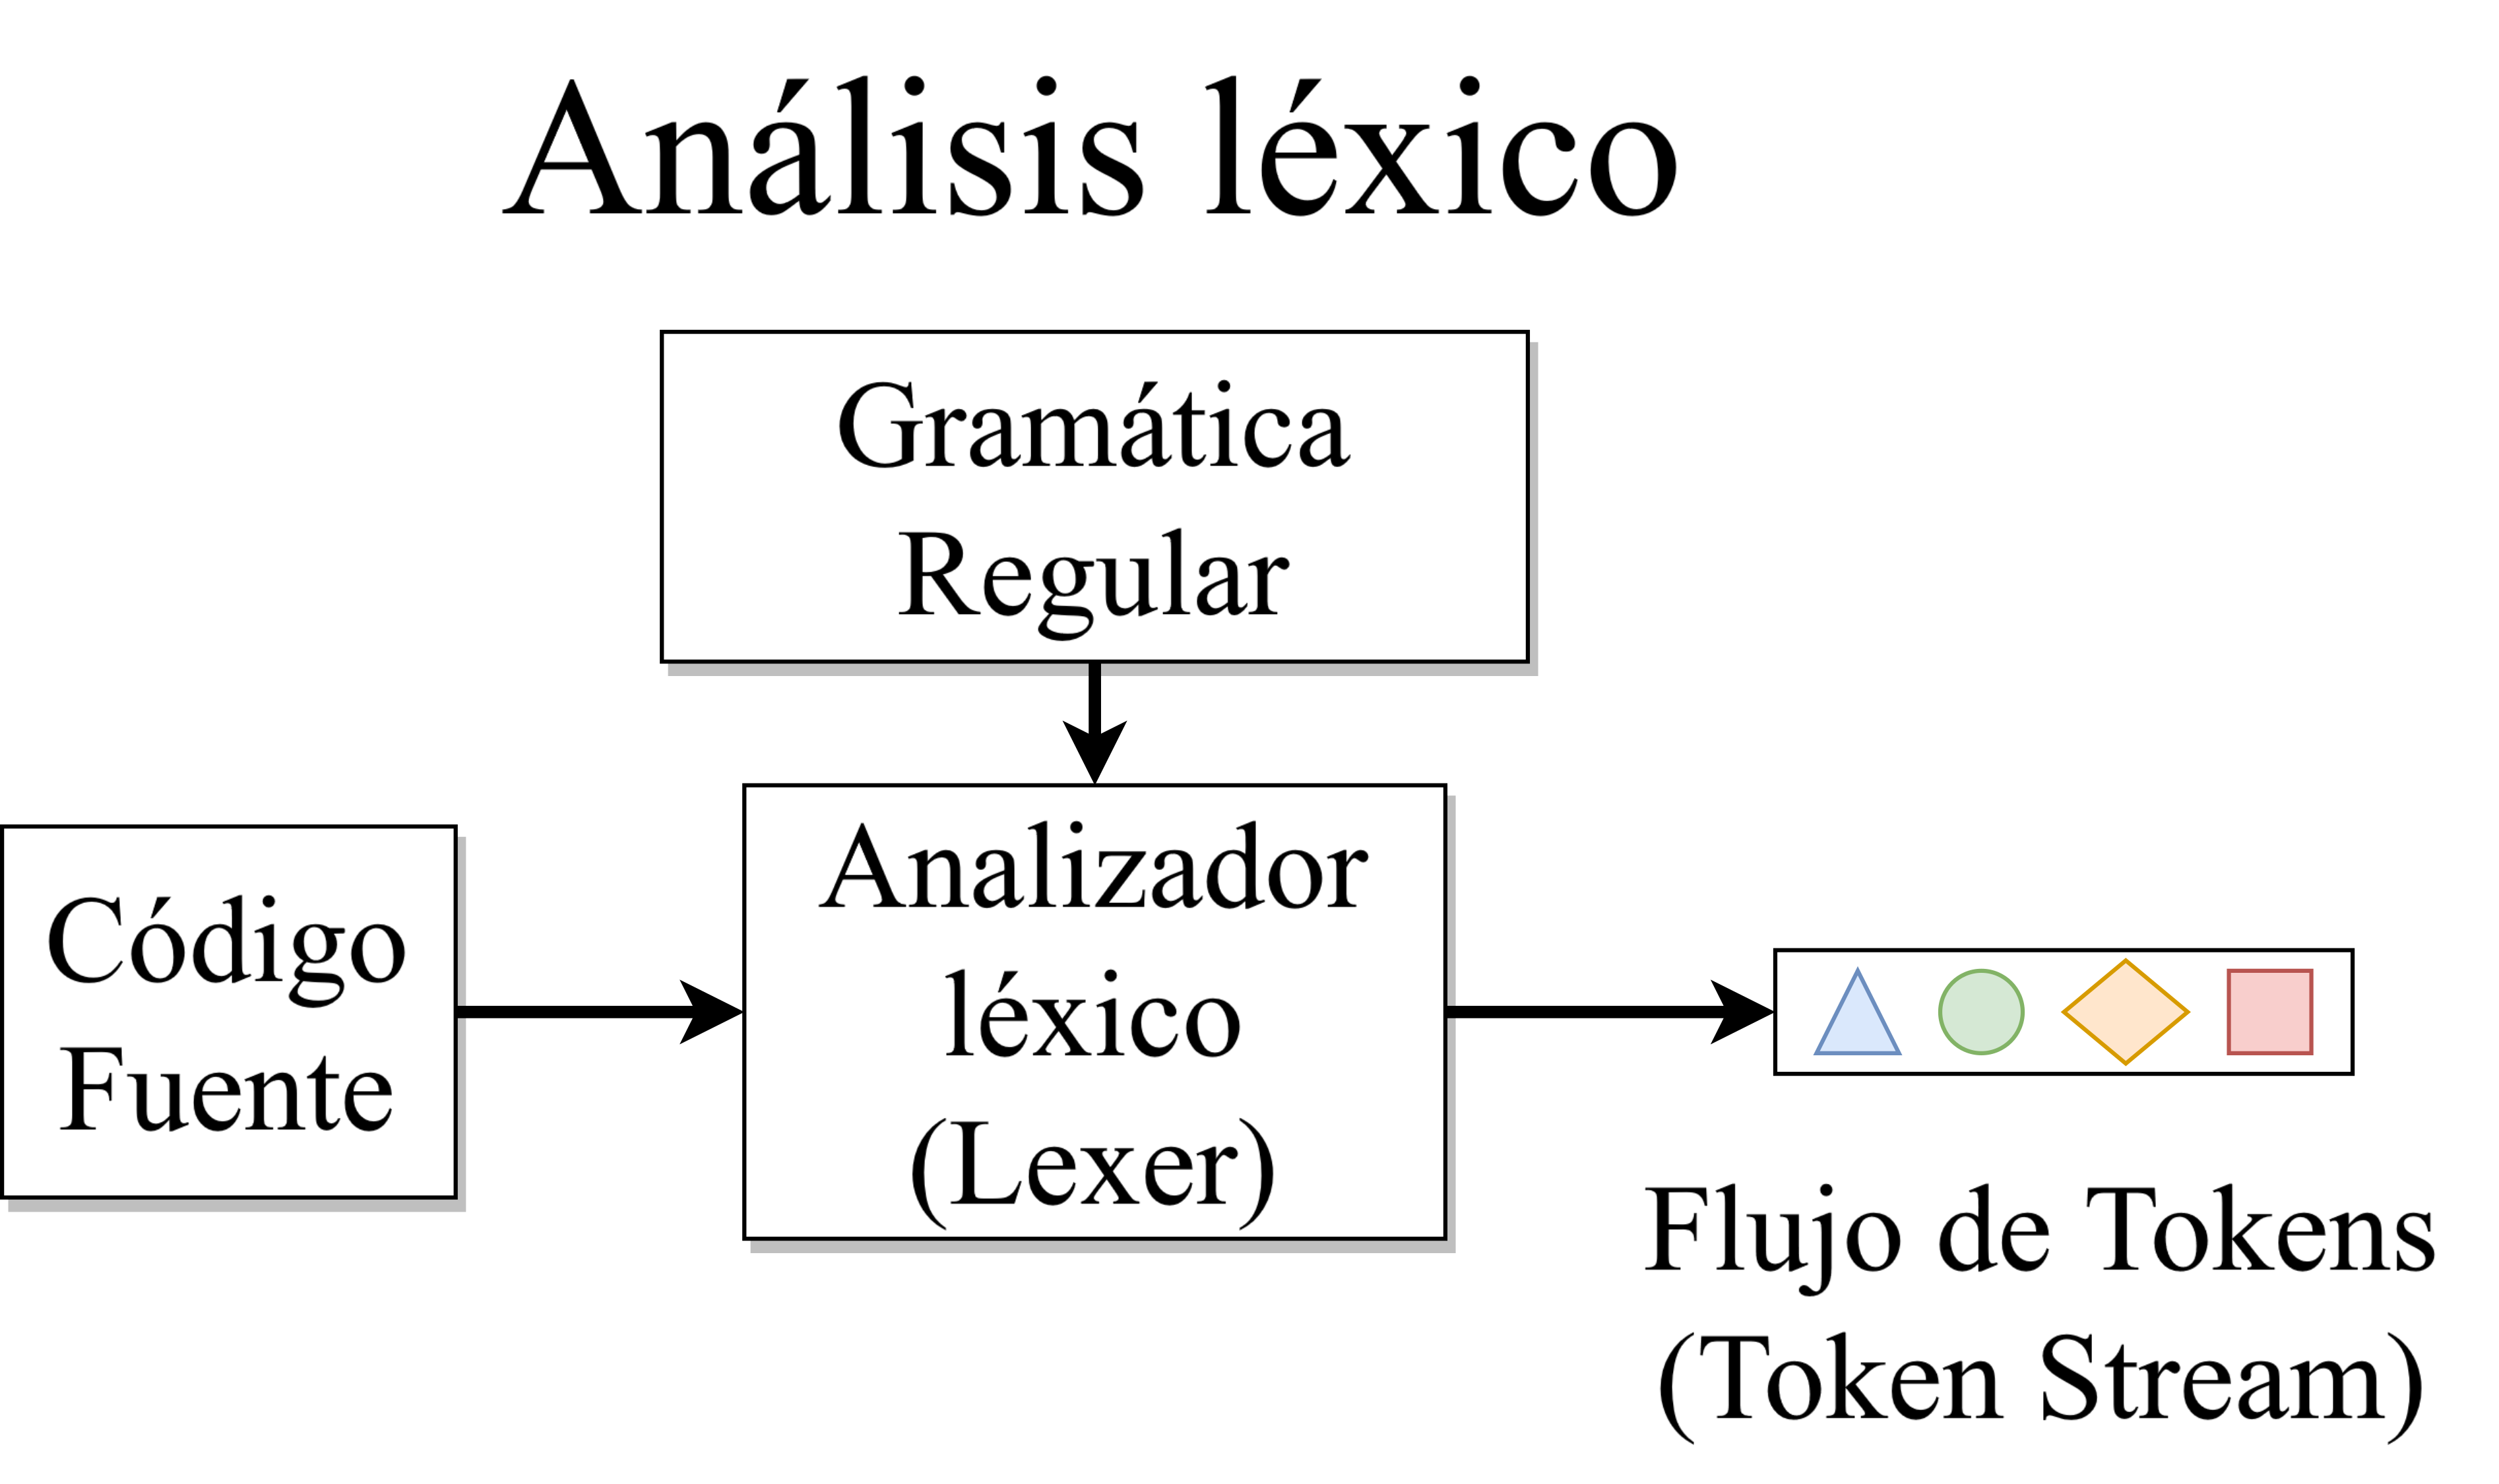
\includegraphics[width=0.8\textwidth]{imagenes/analizadorlexico.png}
	\caption{Funcionamiento del Analizador Léxico en JavaCC\cite{ytanalizadorlexico}}
	\label{fig:analizadorlexico}
\end{figure}

Supongamos que tenemos la siguiente frase: \lstinline|How Pleasant Is The Weather?| . Aquí podemos reconocer fácilmente que hay cinco palabras: “\textit{How}”, “\textit{Pleasant}”, “\textit{Is}”, “\textit{The}” y “\textit{Weather}.” Esto es natural para nosotros, ya que podemos identificar los separadores (espacios en blanco) y el símbolo de puntuación.

Ahora, consideremos una variante de la misma frase: \lstinline|HowPl easantIs Th ewe ather?|. Aquí es donde entra en juego el analizador léxico. Aunque también podemos leer esta versión, llevará más tiempo porque los separadores se colocan en lugares impares. No es algo que se entienda de inmediato.

El analizador léxico escanea el código fuente y reconoce los tokens incluso en situaciones más complejas como esta. En este caso, identificaría las palabras como tokens individuales, a pesar de la falta de espacios.

A continuación se va a ilustrar otro ejemplo, mas orientado a analizar archivos de código. Supongamos un fragmento de código en en un lenguaje de programación ficticio como este:

\lstset{inputencoding=utf8/latin1}
\lstinputlisting{code/lexer.txt}

En este caso, el analizador léxico se encargaría de escanear este código fuente y dividirlo en tokens significativos. El analizador léxico reconocería las palabras clave como \lstinline|suma|, \lstinline|resta|, \lstinline|multiplicacion|, y \lstinline|division|. Además, también identificaría los operadores aritméticos como \lstinline|+|, \lstinline|-|,  \lstinline|*|, y  \lstinline|/|, además de números enteros como  \lstinline|10|,  \lstinline|20|,  \lstinline|30|,  \lstinline|15|,  \lstinline|5|, y \lstinline|6|. Por otra parte, El analizador léxico eliminaría cualquier espacio en blanco o comentario presente en el código. El resultado sería una secuencia de tokens como sigue:

\lstset{inputencoding=utf8/latin1}
\lstinputlisting{code/lexerresultado.txt}

\section{Token}
Un token es una unidad léxica o componente básico del código fuente de un programa. Se trata de una cadena de caracteres con un significado específico asignado. Está estructurado como un par que consta de un nombre de token y un valor de token opcional. El nombre del token representa una categoría o tipo de unidad léxica, como palabras clave, identificadores, operadores, entre otros\cite{token}.

En el ejemplo de la sección anterior, el analizador léxico generaba una secuencia de tokens, cada token tenía sus características propias, dependiendo de si eran identificadores, operadores o signos de puntuación, u otros ---se pueden especificar token que hagan referencias a comentarios dentro del código, o palabras reservadas del lenguaje, como \lstinline[keywordstyle=\color{black}]|if| o \lstinline[keywordstyle=\color{black}]|while|---.


\section{Analizador Sintáctico o Semántico}
Un \textbf{analizador sintáctico} es una parte fundamental de un \textbf{compilador} o intérprete. Su función es verificar si un programa fuente ---escrito en un lenguaje de programación--- sigue las reglas gramaticales definidas para ese lenguaje\cite{analizadorsintactico}. En otras palabras, nos indica la disposición correcta de los elementos en el código fuente para que se convierta en un programa válido.

Comúnmente conocido como \textit{parser}, el analizador sintáctico verifica la \textbf{estructura} del programa fuente. Este hace uso de una gramática (generalmente una gramática libre de contexto) para definir las reglas sintácticas del lenguaje. El objetivo del parser es reconocer la secuencia de \textit{tokens} (unidades léxicas como palabras clave, identificadores, operadores) y construir un \textbf{árbol sintáctico} que represente la estructura jerárquica del programa. Si el archivo fuente es válido, el analizador sintáctico proporciona el árbol sintáctico correspondiente.

Además de todas las funciones mencionadas, si encuentra errores sintácticos, como paréntesis desequilibrados o expresiones mal formadas, el analizador sintáctico genera mensajes de error\cite{traductorescompiladoreseinterpretes}. De esta forma ayuda a los programadores a identificar y corregir problemas en el código fuente de una manera sencilla y muy efectiva. Otras funciones que los analizadores sintácticos pueden desempeñar son el acceder a la tabla de símbolos, ya que necesita información sobre variables, funciones y otros símbolos definidos en el programa; el chequeo de tipos, ya que a menudo se verifica la compatibilidad de tipos ---por ejemplo, si se está aplicando un operador a operandos compatibles--- ; y la generación de código intermedio, proporcionando así una representación más abstracta y simplificada del programa.

\begin{figure}[H]
	\centering
	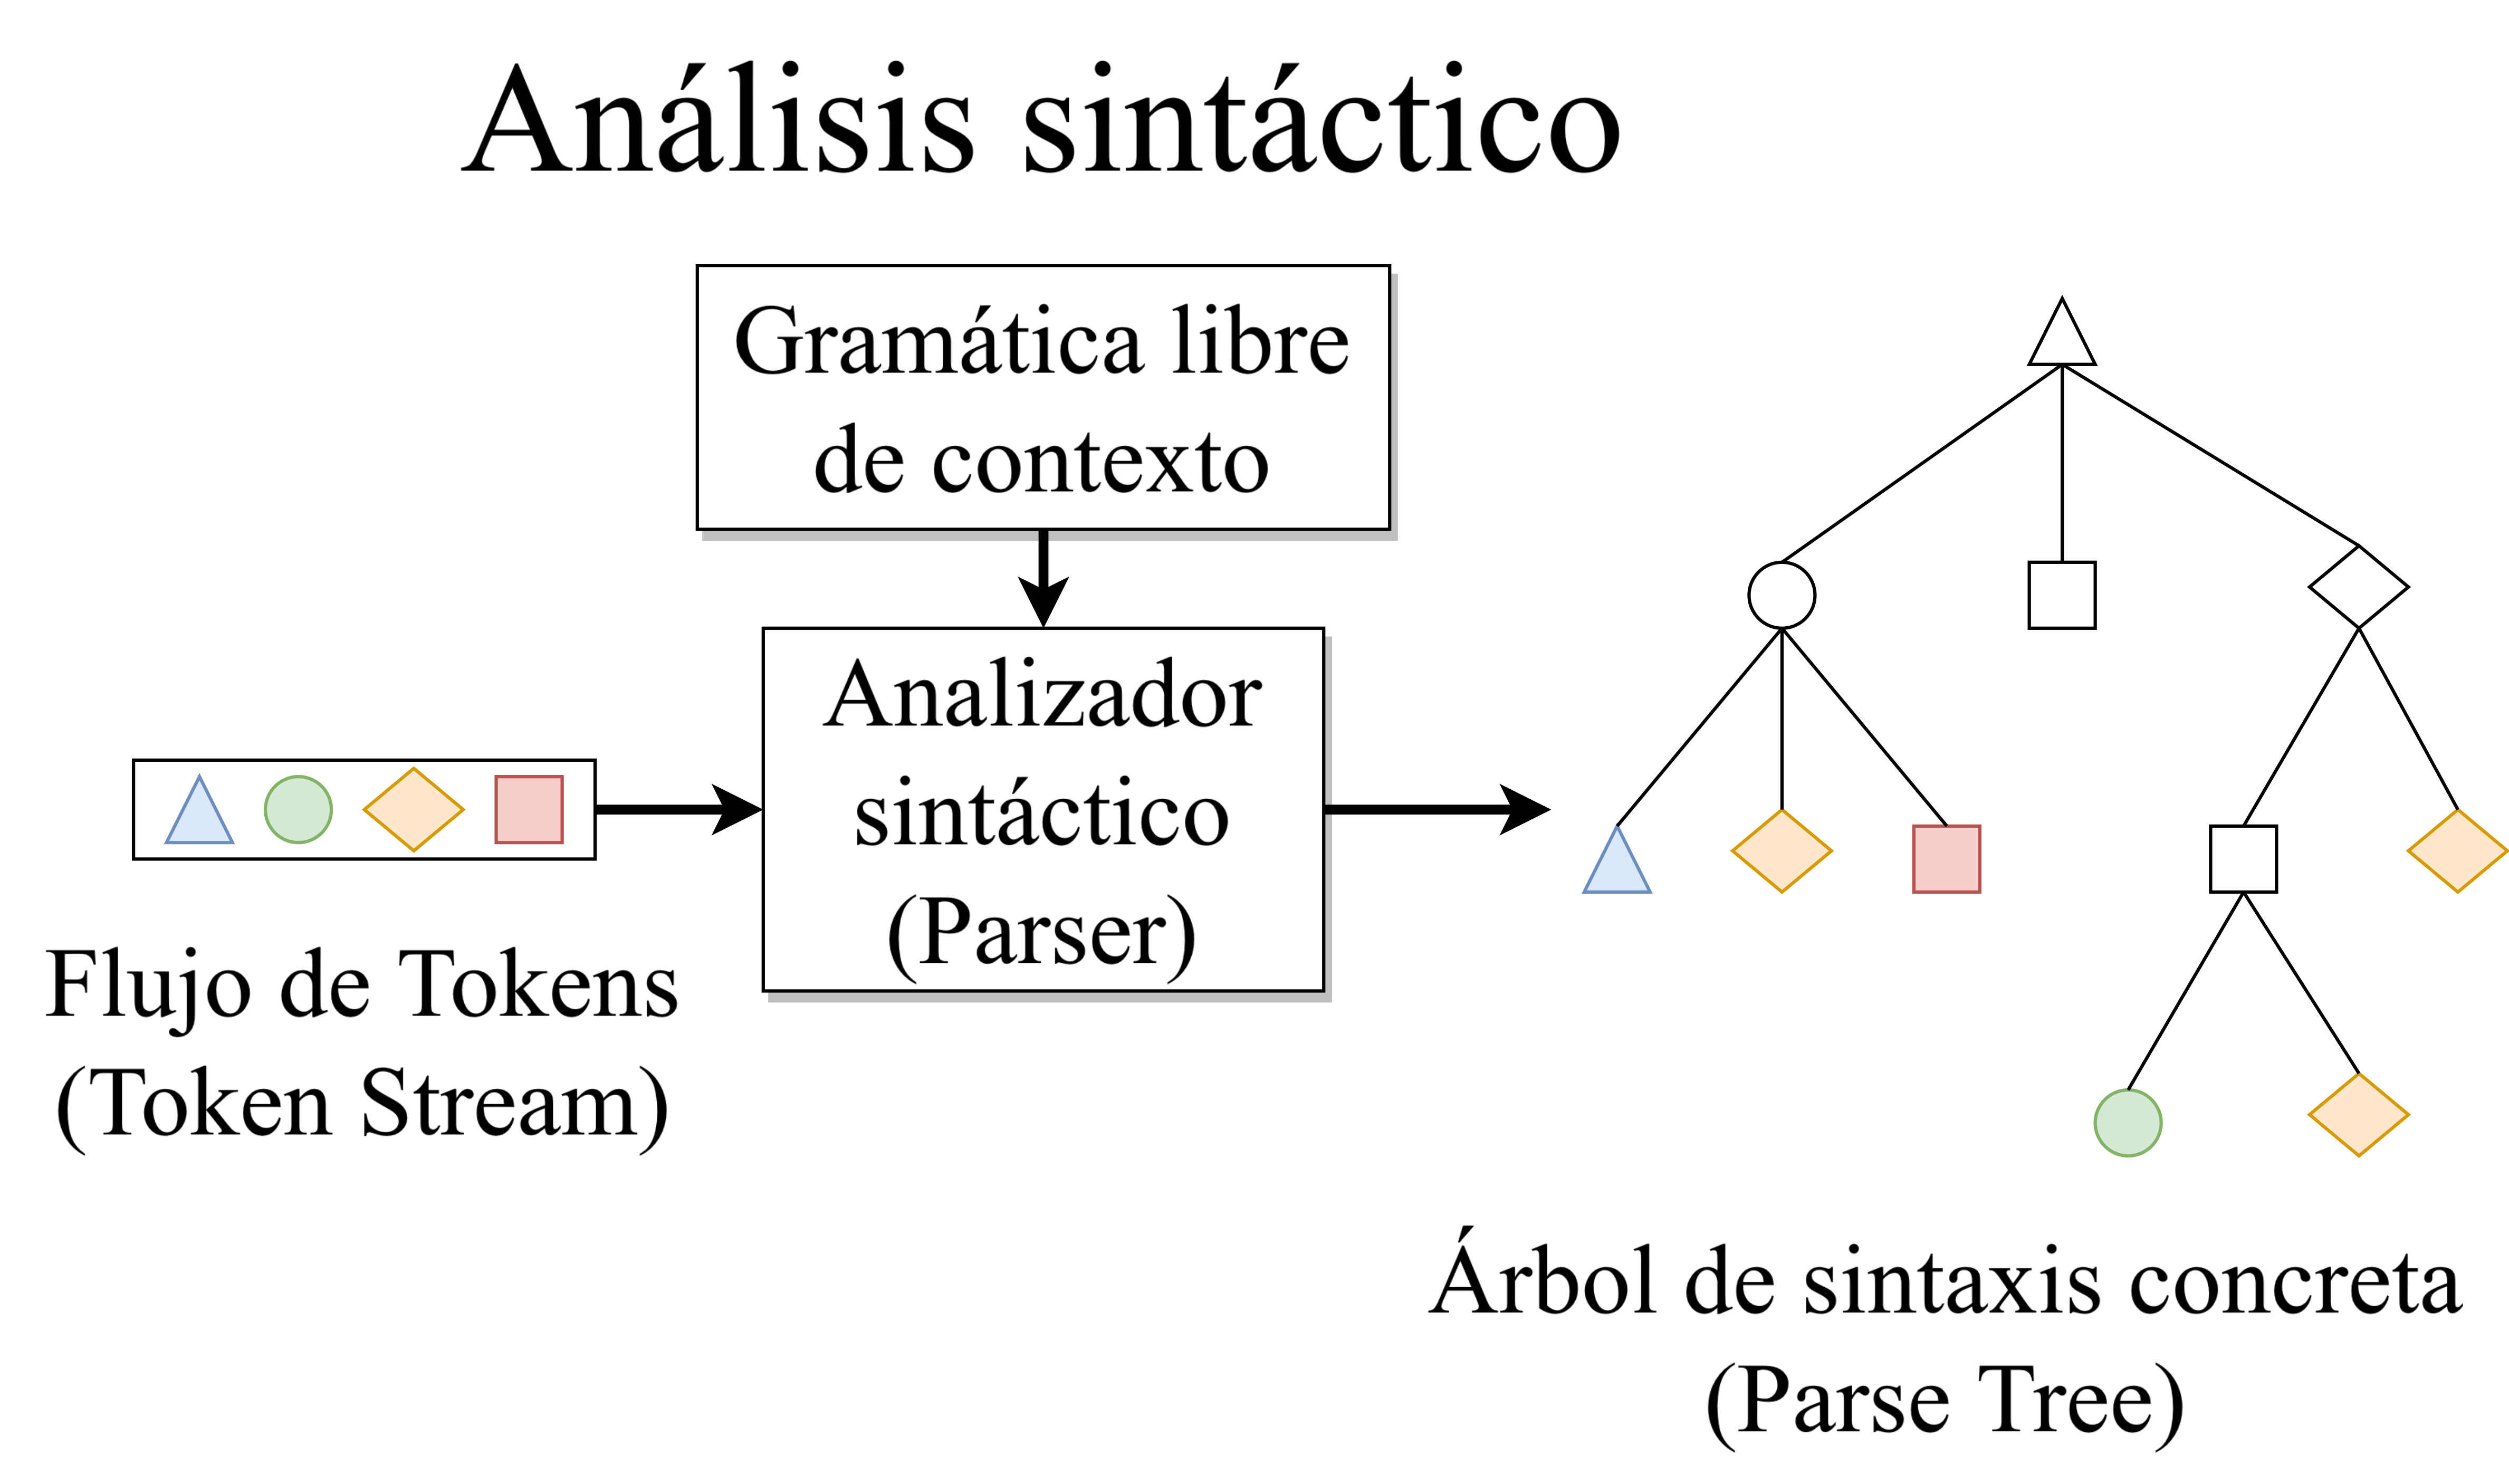
\includegraphics[width=\textwidth]{imagenes/analizadorsintactico.png}
	\caption{\label{fig:analizadorsintactico}Funcionamiento del Analizador Sintáctico en JavaCC\cite{ytanalizadorsintactico}}
\end{figure}



\section{Estados Léxicos}
Los estados léxicos permiten efectuar un conjunto diferente de producciones de expresiones regulares en un caso concreto. Dicho de otra manera, los estados léxicos sirven para que un token este definido de una forma, y en cierto momento del análisis, pueda estar definido de otra forma.

Supongamos que desea escribir un procesador JavaDoc para extraer los comentarios JavaDoc de un documento. La mayor parte de Java está tokenizada de acuerdo con las reglas ordinarias regulares de Java. Pero dentro de los comentarios JavaDoc, se aplica un conjunto diferente de reglas en las que las palabras clave deben ser reconocidas y donde las nuevas líneas son significativas ---como las palabras y símbolos \lstinline|/***/| , \lstinline|@param|, entre otros---.

Para resolver este problema, podríamos usar dos estados léxicos: uno para la tokenización regular de Java y otro para la tokenización dentro de los comentarios de JavaDoc.

\section{Recursividad}

En el ámbito de los compiladores, la recursividad es una técnica que se utiliza para definir una estructura gramatical que se repite en sí misma.

Esto permite resolver problemas complejos dividiéndolos en subproblemas más pequeños. Este proceso se repite hasta que se llega a subproblemas que son triviales de resolver.

En JavaCC, la recursividad se utiliza para definir producciones gramaticales que pueden analizar expresiones complejas.

\subsection{Recursividad a derechas (LR)}
En la recursividad a derechas, la llamada recursiva se realiza al final de la definición de la estructura gramatical. Por ejemplo, la gramática para la expresión aritmética básica se puede definir recursivamente a la derecha de la siguiente manera:

\lstset{inputencoding=utf8/latin1}
\lstinputlisting{code/LR.jj}

\subsection{Recursividad a izquierdas (LL)}

En la recursividad a izquierdas, la llamada recursiva se realiza al principio de la definición de la estructura gramatical. Por ejemplo, la gramática para la expresión aritmética básica se puede definir recursivamente a la izquierda de la siguiente manera:

\lstset{inputencoding=utf8/latin1}
\lstinputlisting{code/LL.jj}



\subsection{¿Por qué no se puede utilizar la recursividad a izquierdas en JavaCC?}
La clase de analizador sintáctico producida por JavaCC funciona por descenso recursivo. La recursión a la izquierda está prohibida para evitar que las subrutinas generadas se llamen a sí mismas recursivamente de forma infinita.

Si considerásemos una producción recursiva a la izquierda, en caso de que la  condición fuera verdadera alguna vez, tendríamos una recursión infinita.
JavaCC producirá un mensaje de error si tiene producciones recursivas a la izquierda.

\section{JavaCC}
En relación con lo anterior, aclaremos a qué hace referencia el concepto de JavaCC y los analizadores semánticos y sintácticos, y como se interrelacionan:
Java Compiler Compiler, comúnmente conocido como JavaCC, es una poderosa herramienta ampliamente utilizada para generar analizadores sintácticos en aplicaciones Java. Su función principal es transformar una especificación gramatical en un programa Java capaz de reconocer y analizar la sintaxis según la gramática proporcionada.
JavaCC se diferencia de otras herramientas similares al generar analizadores sintácticos de arriba hacia abajo ---descenso recursivo, o LL--- en lugar de analizadores de abajo hacia arriba. Esta característica permite el uso de gramáticas más generales y facilita la depuración, además de permitir el análisis en cualquier elemento no terminal de la gramática y la transferencia de valores (atributos) en ambas direcciones en el árbol de análisis.

\section{Funciones principales de JavaCC}
JavaCC ofrece una serie de características y funcionalidades clave que lo hacen destacar como un generador de analizadores sintácticos:
\begin{itemize}
	\item Generación de analizadores sintácticos de arriba hacia abajo.
	\item Resolución de ambigüedades de cambio de turno localmente.
	\item Generación de analizadores 100\% Java puro.
	\item Especificaciones BNF extendidas.
	\item Integración de especificaciones léxicas y gramaticales en un solo archivo.
	\item Manejo de la entrada Unicode completa.
	\item Soporte para tokens no distinguibles entre mayúsculas y minúsculas.
	\item Herramientas adicionales como JJTree para construir árboles y JJDoc para generar documentación.
	\item Personalización a través de numerosas opciones.
	\item Informes de errores de alta calidad y mensajes de diagnóstico completos.
\end{itemize}

\section{Ejemplo de gramática en JavaCC}
A continuación, se presenta un ejemplo de cómo JavaCC puede utilizarse para generar un analizador sintáctico en Java. En este ejemplo se define un lenguaje para analizar expresiones matemáticas simples. Partiendo de este ejemplo, seremos capaz de ampliar las funcionalidades del programa, y realizar una calculadora. El resultado final se encuentra en el archivo \hyperref[sec:mathexp]{Mathexp.jj}, que se encuentra en el apéndice \hyperref[sec:codigofuente]{\textit{Código fuente}}.


\textbf{Función Expression()}

\lstset{inputencoding=utf8/latin1}
\lstinputlisting{code/expression.jj}

La función \textit{Expression()} define la estructura general de una expresión. Una expresión consiste en un término seguido de cero o más términos conectados por operadores aritméticos. La función Expression() comienza con la función Term(). Esto significa que la primera parte de cualquier expresión debe ser un término. A continuación, la función Expression() utiliza la regla )* para especificar que puede seguir cero o más términos. Esto significa que las expresiones pueden tener cualquier longitud, desde una sola palabra hasta una expresión compleja con muchos términos.
Los términos están conectados por operadores aritméticos. La regla Expression() utiliza la regla )* para especificar que puede seguir cualquier número de operadores aritméticos. Esto significa que las expresiones pueden tener cualquier cantidad de operadores aritméticos, desde ninguno hasta muchos. Para más información acerca de operadores en JavaCC, vaya al anexo \hyperref[sec:simbolosdeexpresionesregulares]{\textit{Símbolos de Expresiones regulares en JavaCC}}.
Los operadores aritméticos permitidos son la suma (+), la resta (-), la multiplicación (*) y la división (/).

\textbf{Función Term()}
\lstset{inputencoding=utf8/latin1}
\lstinputlisting{code/term.jj}

La regla \textit{Term()} define la estructura de un término. Un término consiste en un factor seguido de cero o más factores conectados por operadores aritméticos. La regla \textit{Term()} comienza con la regla \textit{Factor()}. Esto significa que la primera parte de cualquier término debe ser un factor. A continuación, la regla \textit{Term()} utiliza la regla \lstinline|)*| para especificar que puede seguir cero o más factores. Esto significa que los términos pueden tener cualquier longitud, desde una sola palabra hasta un término complejo con muchos factores.
Los factores están conectados por operadores aritméticos. La regla \textit{Term()} utiliza la regla \lstinline|)*| para especificar que puede seguir cualquier número de operadores aritméticos. Esto significa que los términos pueden tener cualquier cantidad de operadores aritméticos, desde ninguno hasta muchos.
Los operadores aritméticos permitidos son la suma \lstinline|+|, la resta \lstinline|-|, la multiplicación \lstinline|*| y la división \lstinline|/|

\textbf{Función Factor()}
\lstset{inputencoding=utf8/latin1}
\lstinputlisting{code/factor.jj}
La regla \textit{Factor()} define la estructura de un factor. Un factor puede ser un número o una expresión entre paréntesis. La regla \textit{Factor()} tiene dos opciones. La primera opción es un número. La segunda opción es una expresión entre paréntesis. Si la opción elegida es un número, la regla \textit{Factor()} utiliza la regla \lstinline|<NUMBER>| para especificar que el factor debe ser un número. Si la opción elegida es una expresión entre paréntesis, la regla Factor() utiliza la regla ``('' \textit{Expression()} ``)'' para especificar que la expresión debe estar entre paréntesis.

\textbf{Ejemplos}

Aquí hay algunos ejemplos de expresiones que pueden ser analizadas por esta gramática:

\begin{center}
	\lstinline|1 + 2|

	\lstinline|3 * 4|

	\lstinline|(5 - 6) / 7|
\end{center}

Aunque también se puede analizar expresiones más complejas, como:
\begin{center}
	\lstinline|(1 + 2) * (3 - 4)|

	\lstinline|(5 * 6) / (7 + 8)|
\end{center}

\textbf{Ampliación de la funcionalidad a Calculadora}

A continuación, vamos a ampliar las capacidades de nuestro programa, para analizar las expresiones y hacer las operaciones de una calculadora: \hyperref[sec:nlxlator]{NL\_Xlator.jj}

%\lstset{inputencoding=utf8/latin1}
%\lstinputlisting{code/NL_Xlator.jj}

Esta clase traduce expresiones matemáticas válidas en sus valores numéricos correspondientes. El usuario puede ingresar las expresiones matemáticas una por una, separándolas por punto y coma. La clase lee las expresiones del flujo de entrada estándar y las traduce a sus valores numéricos correspondientes. El resultado de la traducción se muestra en la salida estándar.

\textbf{Análisis sintáctico}

La clase utiliza JavaCC para analizar las expresiones matemáticas ingresadas por el usuario. JavaCC es una herramienta de generación de analizadores de sintaxis que permite crear analizadores personalizados para lenguajes de programación o lenguajes de dominio específicos.

\textbf{Expresión raíz}

La expresión raíz de la gramática es \textit{ExpressionList()}. Esta producción analiza una lista de expresiones matemáticas separadas por punto y coma. Cada expresión matemática es analizada por la producción Expression().

\textbf{Expresión}

La producción \textit{Expression()} analiza una expresión matemática completa. Esta producción analiza un término (Term()) seguido de cero o más operadores de suma o resta (+ o -) y términos.

\textbf{Término}

La producción \textit{Term()} analiza un término matemático. Esta producción analiza un factor (\textit{Factor()}) seguido de cero o más operadores de multiplicación o división (* o /) y factores.

\textbf{Factor}

La producción \textit{Factor()} analiza un factor matemático. Esta producción analiza un número (NUM) o un par de paréntesis ((, )) que encierran una expresión matemática.

\textbf{Errores}

La clase también maneja errores sintácticos. Cuando ocurre un error sintáctico, la clase muestra un mensaje de error en la salida estándar y termina la ejecución.

\textbf{Ejemplo de uso}

Para utilizar la clase, simplemente ejecute el archivo NL\_Xlator.java. A continuación, se le pedirá que ingrese expresiones matemáticas una por una, separándolas por punto y coma. La clase le mostrará el resultado de la traducción de cada expresión.
Aquí hay un ejemplo de cómo utilizar la clase:

\section{Usos de JavaCC en la actualidad}

JavaCC es una herramienta muy completa a la hora de construir de analizadores léxicos y sintácticos para lenguajes de programación. Si bien su desarrollo original se centró en Java, su flexibilidad y robustez lo han convertido en una herramienta versátil con aplicaciones en diversos campos.

En el contexto de los lenguajes de programación, JavaCC ha tenido varias aplicaciones, como es el caso de Apache. A modo de ejemplo del proyecto Apache, JavaCC se utiliza en el proyecto Apache Ant para analizar archivos  \lstinline|build.xml|, que definen las tareas de construcción de software\cite{apache}, aunque indagaremos en unos momentos en el proyecto Apache. Por otro lado, JavaCC se ha utilizado para construir compiladores e intérpretes para diversos lenguajes de programación, como Python, Ruby, C\#, PHP, y JavaScript\cite{javaccc++preprocessor}.

Otra aplicación en la que JavaCC se puede desenvolver con comodidad es el análisis del lenguaje natural. JavaCC se utiliza para analizar la estructura sintáctica de oraciones en aplicaciones de procesamiento de lenguaje natural\cite{languageprocessing}. También se utiliza para extraer información de documentos de texto, como nombres de entidades, fechas y lugares.

Si nos centramos en el marco actual, hay un gran repertorio de aplicaciones comerciales que hacen uso de JavaCC. Un buen ejemplo de ello es el proyecto de Apache.

\textbf{Apache}

Apache Software Foundation es una comunidad descentralizada de desarrolladores que trabajan en sus propios proyectos de código abierto. Los proyectos Apache se caracterizan por un modelo de desarrollo basado en el consenso, la colaboración y una licencia de software abierta y pragmática\cite{apachepaginaoficial}. Uno de los proyectos notables dentro de la Apache Software Foundation es el servidor web Apache HTTP, que consiste en un servidor web HTTP de código abierto utilizado para crear páginas y servicios web. Es multiplataforma, gratuito, robusto y se destaca por su seguridad y rendimiento\cite{apachehttp}.

Entre los proyectos Apache en los que JavaCC se utiliza, cabe destacar Apache Lucene --- en el que se emplea para procesar consultas, permitiendo interpretar y procesar estructuras gramaticales definidas en lenguajes específicos---, Apache Avro ---que trasforma lenguajes de alto nivel a esquemas Avro--- , o por ejemplo Apache Tomcat ---que parsea expresiones de lenguaje (\textit{Expression Language})\cite{expressionlanguage} y JSON--- \cite{javaccgithub}.

Como se ha mencionado antes, en el proyecto de Apache Ant se utiliza JavaCC para analizar archivos \lstinline|build.xml|. JavaCC se encarga de analizar la sintaxis del archivo y construir un árbol de sintaxis, mientras que Ant coordina y automatiza las tareas de construcción y despliegue.

JavaCC también se utiliza en el parseo de archivos desarrollados en Java, como puede ser la librería JavaParser\cite{javaparser}. Otros proyectos en los que se utilice JavaCC, aparte de Apache, son JFlex y ANTLR.

\textbf{JFlex}

JFlex es una herramienta para la construcción de analizadores léxicos. Este está escrito en Java y se utiliza junto con JavaCC para analizar la sintaxis de las reglas léxicas. Por una parte, JFlex se encarga de generar el analizador léxico que escanea el código fuente y produce tokens. Posteriormente, se utiliza JavaCC para generar el analizador sintáctico que procesa los tokens generados por el escáner léxico y aplica las reglas gramaticales

\textbf{ANTLR}

ANTLR (\textit{ANother Tool for Language Recognition}) es una herramienta para la construcción de analizadores léxicos y sintácticos. En términos de funcionalidades, es una herramienta más completa que abarca tanto el análisis léxico como el sintáctico. Sin embargo, JavaCC es más rápido y más fácil de aprender para un desarrollador Java, ya que la sintaxis es muy parecida, ademas de que ofrece una buena integración con IDEs\cite{antlr}. Además de generar analizadores sintácticos, también crea analizadores léxicos (escáneres) y árboles de sintaxis abstracta (AST).
ANTLR está escrito en Java y se puede utilizar junto con JavaCC para analizar la sintaxis de las gramáticas.

\section{Procesamiento de la Información en Aplicaciones Telemáticas (PIAT)}
\subsection{Introducción}
Las prácticas de PIAT son una serie de ejercicios que se utilizan para enseñar a los estudiantes de la asignatura los fundamentos de la programación orientada a objetos, y como se puede utilizar para analizar y extraer información de distintos formatos. Estas prácticas incluyen ejercicios de análisis de ficheros XML y JSON, principalmente.

La aplicación de JavaCC en las prácticas de PIAT tiene varias ventajas potenciales. En primer lugar, puede ayudar a los estudiantes a aprender los fundamentos de la programación orientada a objetos de una manera más eficiente y de una forma que todavía no han tenido la oportunidad de aprender y explotar. En segundo lugar, puede ayudar a los estudiantes a desarrollar sus habilidades de programación, y por consecuencia, ayudar a los estudiantes a crear código más eficiente y de mejor calidad.
\subsection{Problemática con las prácticas de PIAT}

Las prácticas de PIAT, que se centran en el análisis de archivos XML o JSON,  utilizan soluciones como SAXParser o XPath ---las veremos en detalle mas adelante---. Estas soluciones, sin embargo, presentan una serie de problemas que pueden dificultar el desarrollo de código eficiente y mantenible.

Uno de los principales problemas de SAXParser y XPath es que generan mucho código repetitivo. Los bucles while y loops que se utilizan para recorrer el árbol de datos pueden ser muy largos y complejos, lo que dificulta la comprensión y el mantenimiento del código.

Otro problema de estas soluciones es que pueden ser ineficientes en el rendimiento. SAXParser, por ejemplo, se basa en un modelo de eventos, lo que significa que el código debe estar preparado para procesar cualquier tipo de evento que pueda ocurrir. Esto puede provocar que el código se ejecute de forma innecesaria, lo que puede afectar al rendimiento de la aplicación.

Una buena solución a este tipo de soluciones es un generador de analizadores sintácticos como JavaCC. JavaCC permite crear analizadores sintácticos a partir de una gramática definida por el usuario. Esto permite generar código más eficiente y fácil de mantener, ya que el analizador sintáctico se genera automáticamente a partir de la gramática.

Al definir la gramática del analizador sintáctico de forma personalizada, este ofrece una gran flexibilidad, ya que permite adaptar el analizador a las necesidades específicas de la aplicación. Por ejemplo, si queremos analizar un archivo XML que tiene una estructura específica, podemos definir una gramática que refleje esa estructura. Esto nos permitirá generar un analizador que sea más eficiente y fácil de mantener.

Además, una vez que se ha definido la gramática, JavaCC genera el código fuente del analizador sintáctico. Este código fuente se puede modificar a conveniencia, lo que nos permite adaptar el analizador a las necesidades específicas de la aplicación. Esto permite que, si queremos añadir nuevas funcionalidades al analizador, podemos hacerlo fácilmente modificando el código fuente. Esto nos permite tener un mayor control sobre el analizador y adaptarlo a las necesidades cambiantes de la aplicación, característica clave en el entorno de las practicas de PIAT, ya que se caracterizan por tener un estilo incremental y con modificaciones a lo largo de cada ejercicio.

Por otra parte, si bien es cierto que JavaCC puede ser una herramienta compleja para aprender a utilizar, ya que requiere un conocimiento básico de gramáticas y de la sintaxis de Java, el potencial que ofrece JavaCC para desarrollar analizadores sintácticos eficientes y adaptables es muy alto.

Una vez se ha aprendido a utilizar JavaCC, se puede utilizar para desarrollar analizadores sintácticos para una amplia gama de lenguajes, incluyendo XML, JSON, HTML, C++, PHP, Cobol, SQL, IDL, entre otros\cite{javaccgithub}.

\chapter{Desarrollo}
\label{sec:cap3}
\section{Introducción}
En el capítulo anterior se han expuesto las principales tecnologías que forman parte del proyecto de evaluación de la viabilidad de JavaCC para el procesamiento de información en la asignatura PIAT. En este capítulo se desarrollarán los aspectos relativos a la implementación del proyecto, los procedimientos seguidos y el entorno utilizado para los desarrollos y las pruebas.

\section{Implementación}
La implementación del proyecto se ha realizado en Java, utilizando la herramienta JavaCC para la generación de los analizadores léxico y sintáctico. Para la creación de las gramáticas se ha utilizado el lenguaje EBNF.

\section{Procedimientos}

El proceso de implementación se ha dividido en las siguientes fases:
\begin{itemize}
    \item Fase 1: Aprendizaje de los conceptos básicos de JavaCC.
    \item Fase 2: Práctica con JavaCC para crear analizadores léxicos y sintácticos para gramáticas simples.
    \item Fase 3: Aplicación de JavaCC en prácticas de PIAT.
    \item Fase 4: Generación de documentación.
\end{itemize}

\section{Entorno}
Los desarrollos y las pruebas se han realizado en un entorno de desarrollo integrado (IDE) de Java. En concreto, se ha empleado Eclipse IDE ya que, además de ser el IDE principal con el que se realizan las prácticas de PIAT ---y en general, cualquier práctica relacionada con la programación dentro de la escuela---, existe un plugin de JavaCC que realiza la compilación de los archivos y facilita enormemente el desarrollo. Para la depuración de los analizadores se ha utilizado el debugger del IDE.

Para saber mas acerca de la instalación y configuración de Elipse IDE con JavaCC, puede consultar el anexo \hyperref[sec:instalaciondejavacc]{\textit{Instalación de JavaCC}}.

\section{Objetivos de la implementación}
Entre los objetivos principales de la implementación se encuentran el implementar los analizadores léxico y sintáctico para las gramáticas de las prácticas de PIAT, el evaluar la viabilidad de utilizar JavaCC para abordar las prácticas de PIAT, y generar documentación que sirva como recurso para estudiantes y profesores interesados en utilizar JavaCC en proyectos relacionados con el procesamiento de información.

\section{Conclusiones}
En esta sección se ha presentado una introducción al desarrollo de la propuesta. En las siguientes secciones se desarrollarán los aspectos relativos a la implementación, los procedimientos seguidos y el entorno utilizado para los desarrollos y las pruebas.

\section{Análisis de ficheros de \textit{log}. Práctica 2}
\subsection{Introducción}

\section{Análisis de archivos XML. Práctica 3}
\subsection{Introducción}

La práctica 3 de PIAT, centrada en el procesamiento de documentos XML, representa un hito significativo en el marco de este proyecto. En esta etapa, se aborda la implementación de un analizador de documentos XML utilizando la tecnología SAX. El objetivo principal es familiarizar a los estudiantes con SAX y fortalecer sus habilidades en el diseño de algoritmos eficientes para la extracción y transformación de información a partir de fuentes de contenidos estructurados.
La práctica 3 de PIAT se centra en familiarizarse con la tecnología SAX y desarrollar un analizador de documentos XML basado en esta tecnología. Además, el objetivo secundario es diseñar algoritmos eficientes que permitan la extracción y transformación de información a partir de fuentes de contenidos estructurados.

\subsection{SAX}
La tecnología SAX (Simple API for XML) es una API que se encarga de procesar documentos XML. Está basada en eventos, lo que quiere decir que el analizador XML notifica al programa cuando encuentra un evento especifico en el documento. El programa puede tomar medidas en función del evento. Los eventos que puede notificar SAX son:
\begin{itemize}
    \item Inicio de documento: Se produce cuando el analizador comienza a procesar el documento.
    \item Fin de documento: Se produce cuando el analizador finaliza el procesamiento del documento.
    \item Inicio de elemento: Se produce cuando el analizador encuentra el inicio de un elemento XML.
    \item Fin de elemento: Se produce cuando el analizador encuentra el final de un elemento XML.
    \item Caracteres: Se produce cuando el analizador encuentra caracteres no pertenecientes a un elemento XML.
    \item Error: Se produce cuando el analizador encuentra un error en el documento XML.
\end{itemize}

SAX es una buena opción para procesar documentos XML grandes o complejos. Esto se debe a que el analizador XML no necesita cargar todo el documento en memoria a la vez. En cambio, el analizador puede procesar el documento de forma secuencial, lo que puede ahorrar memoria.

SAX también es una buena opción para procesar documentos XML que se actualizan con frecuencia. Esto se debe a que el analizador XML puede procesar solo los cambios en el documento, lo que puede ahorrar tiempo.

Algunos ejemplos de cómo se puede utilizar SAX para procesar documentos XML incluyen:
\begin{itemize}
    \item Leer un documento XML y extraer los datos que contiene.
    \item Validar un documento XML para asegurarse de que cumple con las reglas de un esquema XML.
    \item Transformar un documento XML a un formato diferente.
\end{itemize}

\subsection{JavaCC vs SAX}

JavaCC y SAX son dos API diferentes para procesar documentos XML. JavaCC es una herramienta de generación de analizadores que permite crear analizadores XML personalizados. SAX es una API estándar que proporciona un conjunto de métodos para procesar documentos XML.
Hay varias razones por las que JavaCC puede ser una mejor opción que SAX para procesar documentos XML:
\begin{itemize}
    \item Control: JavaCC ofrece un mayor control sobre el proceso de análisis que SAX. Esto permite a los desarrolladores crear analizadores que se adapten a sus necesidades específicas.
	\item Eficiencia: JavaCC puede generar analizadores que sean más eficientes que los analizadores SAX estándar. Esto se debe a que JavaCC puede aprovechar las características del lenguaje Java para optimizar el proceso de análisis.
	 \item Flexibilidad: JavaCC permite crear analizadores XML que sean más flexibles que los analizadores SAX estándar. Esto se debe a que JavaCC permite a los desarrolladores definir sus propias reglas de análisis.
\end{itemize}
En concreto, JavaCC ofrece las siguientes ventajas sobre SAX:
\begin{itemize}
    \item Puede generar analizadores personalizados que se adapten a las necesidades específicas del documento XML. Esto permite a los desarrolladores crear analizadores que sean más eficientes, precisos y fáciles de mantener.
    \item Puede generar analizadores que sean más eficientes que los analizadores SAX estándar. Esto se debe a que JavaCC puede aprovechar las características del lenguaje Java para optimizar el proceso de análisis.
    \item Puede generar analizadores que sean más flexibles que los analizadores SAX estándar. Esto se debe a que JavaCC permite a los desarrolladores definir sus propias reglas de análisis.
\end{itemize}

Sin embargo, JavaCC también tiene algunas desventajas con respecto a SAX:
\begin{itemize}
    \item Es más complejo de aprender y usar que SAX. Esto se debe a que JavaCC requiere conocimientos de programación en Java.
    \item Puede ser más lento que SAX para documentos XML pequeños. Esto se debe a que JavaCC debe generar un analizador personalizado para cada documento XML.
\end{itemize}

En general, JavaCC es una buena opción para procesar documentos XML cuando se necesita un mayor control, eficiencia o flexibilidad. Sin embargo, SAX es una buena opción para procesar documentos XML pequeños o cuando se necesita una solución rápida y fácil de usar.

\subsection{Descripción de la práctica}

A continuación se presenta el enunciado de la práctica propuesta del año 2022:
Se desea desarrollar una aplicación que extraiga cierta información de un fichero XML obtenido a partir de los datos publicados en el Portal de Datos Abiertos del Ayuntamiento de Madrid (http://datos.madrid.es).

La información (organismos, eventos, actividades, …) publicada a través del Portal de Datos Abiertos presenta las siguientes características:

\begin{itemize}
    \item Los elementos de información, en adelante recursos (concept), se identifican mediante una URI.
    \item Cada recurso se encuentra asociado a una categoría (elemento code de concept).
    \item Los recursos se encuentran agrupados en conjuntos de datos (elemento dataset) accesibles en formato JSON a través de un URI indicada en el atributo id del elemento dataset.
    \item En un dataset puede haber información sobre recursos asociados a varias categorías.
    \item Los recursos de una categoría pueden estar accesibles a través de diferentes datasets.
    \item Para la categorización de los recursos se utiliza un sistema de clasificación jerárquico basando en características temáticas.
\end{itemize}

Esta información se encuentra descrita en un Catálogo de Datos en formato XML (\hyperref[sec:catalogoxml]{catalogo.xml}) válido con respecto al esquema \hyperref[sec:catalogoxsd]{catalogo.xsd}.
La aplicación por desarrollar proporcionará una herramienta de búsqueda que posibilite la recuperación de recursos asociados a un código de categoría generando un documento XML con los resultados.
La Figura 1 muestra un ejemplo de presentación de parte de la estructura jerárquica de los concepts del catálogo.

\begin{figure}[H]
\centering
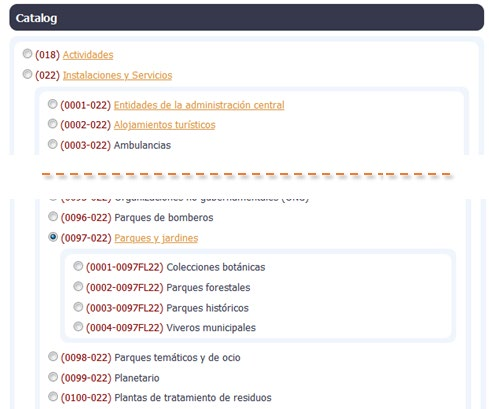
\includegraphics[width=\textwidth]{imagenes/Practica3fig1.jpg}
\caption{\label{fig:Practica3fig1.jpg}Representación de la estructura jerárquica de los concepts del catálogo de datos.}
\end{figure}


La aplicación por desarrollar recibirá como argumento el criterio de búsqueda, esto es, el código de la categoría de la que se desea información, y proporcionará información sobre los concepts y datasets pertinentes, aplicando para ello los siguientes criterios:

\begin{itemize}
    \item Se considerarán pertinentes el concept cuyo código (elemento code) coincida con el criterio de búsqueda y todos los concepts descendientes del mismo.
    \item Se considerarán pertinentes los dataset que contengan información asociada a alguno de los concept pertinentes (contengan un elemento concept con el atributo id igual al atributo id del elemento concept pertinente).
\end{itemize}

La Figura 2 muestra un ejemplo de búsqueda del concept con código 0097-022 y los resultados que se obtendrían.

\begin{figure}[H]
\centering
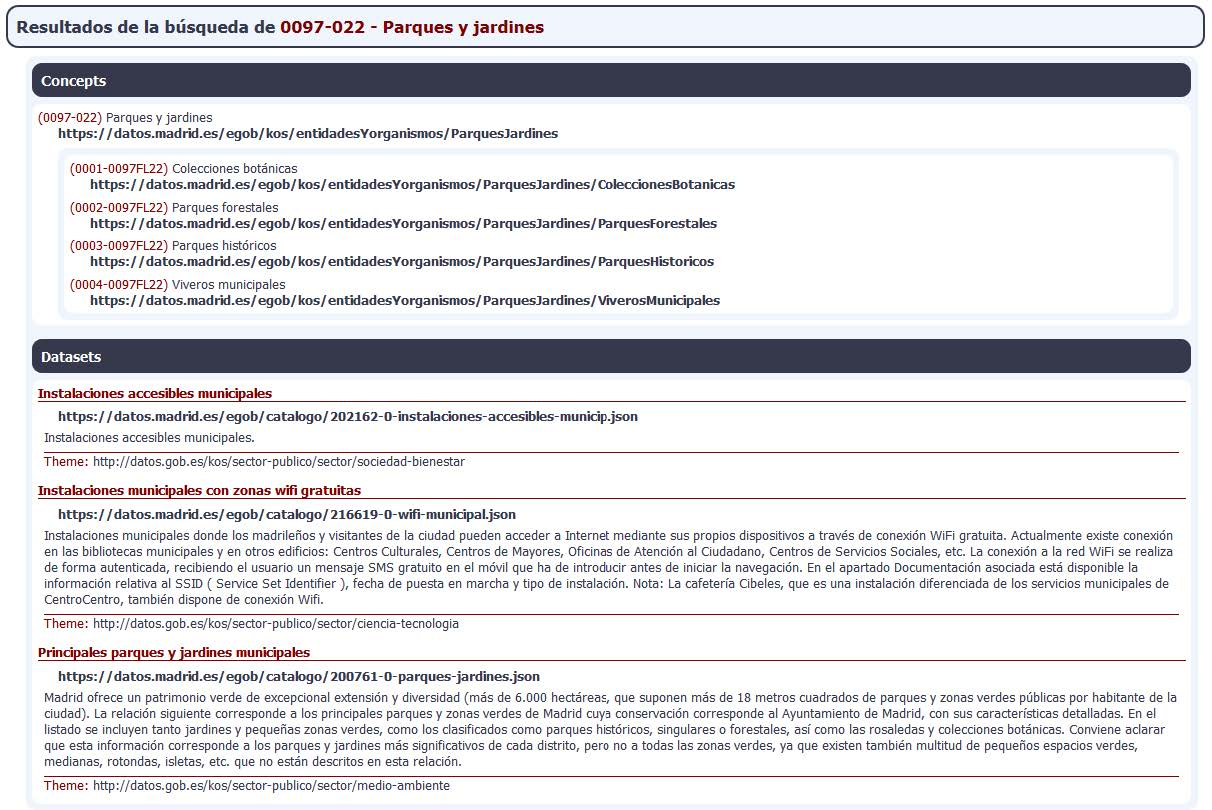
\includegraphics[width=\textwidth]{imagenes/Practica3fig2.jpg}
\caption{\label{fig:Practica3fig2.jpg}Concepts y datasets pertinentes para el código 0097-022.}
\end{figure}

\subsection{Desarrollo de la práctica}

La implementación de la Práctica 3 se basa en la creación de un analizador de documentos XML denominado XMLParser, desarrollado utilizando JavaCC, una herramienta que permite generar analizadores léxicos y sintácticos en el lenguaje Java. Este analizador se ha diseñado para procesar documentos XML que contienen datos publicados en el Portal de Datos Abiertos del Ayuntamiento de Madrid (http://datos.madrid.es).
Los documentos XML que se procesan a través de esta herramienta presentan ciertas características clave, como la identificación de recursos mediante URI, la asociación a categorías, la agrupación en conjuntos de datos y una clasificación jerárquica basada en características temáticas. La tarea principal del analizador es extraer información específica relacionada con códigos de categorías y, posteriormente, generar un nuevo documento XML que contiene los resultados deseados.

\subsection{Herramienta}
La principal herramienta desarrollada en esta práctica es el analizador XMLParser. Este analizador es capaz de llevar a cabo varias tareas esenciales:

\begin{itemize}
    \item Validación de argumentos de entrada para garantizar que los parámetros cumplan con las especificaciones requeridas.
    \item Extracción de información relevante de los documentos XML, siguiendo las reglas y estructuras definidas en la gramática.
    \item Generación de documentos de resultados que cumplen con un esquema específico.
\end{itemize}
El analizador XMLParser representa una contribución significativa en términos de procesamiento y manipulación de documentos XML.


\subsection{Conclusiones}

La Práctica 3 ha brindado a los estudiantes una experiencia valiosa en el manejo de tecnologías de análisis de documentos XML. A través del uso de JavaCC y la tecnología SAX, se ha proporcionado una base sólida para procesar información estructurada de manera eficiente. Los estudiantes han tenido la oportunidad de aplicar conceptos relacionados con la validación de argumentos, el análisis de elementos XML y la generación de documentos de resultados.
Uno de los aspectos más destacados de esta práctica es la capacidad de filtrar y seleccionar información relevante basada en códigos de categorías. Esta habilidad es fundamental en situaciones donde la extracción selectiva de datos es esencial.

\subsection{Preguntas Frecuentes}

¿Qué sentido tiene utilizar la clase ManejadorXML, si el parser ya busca lo que quiere?
Tiene sentido cronologico, ya que primero el parser realiza el analisis del documento y devuelve los datos, si se llama a una funcion que devuelva los datos es posible que se llamen a estas funciones antes de que se llame a la funcion de análisis

\subsection{Notas}

hacer clase concept con atributos code y label, hacer lista concepts de concept. hacer lo mismo con dataset. recoger los datos al igual que haciamos en NXCalculator
Concepts, son objetos distintos, se tienen que reconocer de manera diferente. -> Nuevo objeto conceptInDataset
No hace falta un estado lexico, simplemente crear un objeto nuevo ya que son cosas diferentes, -> IncludedConcepts
String id -> idConcepts
XMLParser devuelve un objeto que tenga implementado la interfax ParserCatalogo


\subsection{Código Fuente}

El código fuente de los archivos elaborados en esta practica se encuentra a continuación para su estudio y aprendizaje. Cabe destacar que se proporcionan dicho código para que el lector sea capaz de probar las funcionalidades con el objetivo de aprender mas acerca de las aplicaciones de JavaCC.

No se promueve el plagio y la realización de las prácticas, este simplemente es una de las muchas formas en las que se podría realizar la práctica.

\hyperref[sec:XMLParser]{XMLParser.jj}
%\href{https://shorturl.at/alqN6}{XMLParser.jj}

\section{Análisis de archivos JSON. Práctica 4}

\subsection{Introducción}

La Práctica 4 se centra en la exploración y aplicación de la tecnología GSON Streaming para el análisis y procesamiento eficiente de documentos JSON. El objetivo principal de esta etapa es familiarizar a los estudiantes con la API GSON Streaming y desarrollar un analizador de documentos JSON basado en esta tecnología. Como objetivo secundario, se busca capacitar a los estudiantes en el diseño de algoritmos eficientes para la extracción y transformación de información proveniente de fuentes de contenidos estructurados.

\subsection{GSON Streaming}

La API de transmisión de GSON es una API de Java que permite leer y escribir JSON de forma secuencial. Esto la hace útil en situaciones donde no es posible o deseable cargar el modelo de objeto completo en memoria, como cuando se trabaja con grandes cantidades de datos o cuando los datos se reciben de forma continua.

La API de transmisión de GSON se basa en dos clases principales: JsonReader y JsonWriter. JsonReader se utiliza para leer JSON de forma secuencial, mientras que JsonWriter se utiliza para escribir JSON de forma secuencial.

Las características principales de la API son su eficiencia en términos de memoria y  su flexibilidad. Por una parte, la API de transmisión de GSON no necesita cargar el modelo de objeto completo en memoria, lo que la hace más eficiente en términos de memoria que la API de GSON tradicional. Además, GSON Streaming permite leer y escribir datos JSON de forma secuencial, lo que la hace muy flexible.

La API es ideal para trabajar con grandes cantidades de datos, ya que puede leer y escribir los datos sin necesidad de cargarlos todos en memoria. También es ideal para recibir datos de forma continua, ya que puede leer los datos a medida que se reciben.


\subsection{JavaCC vs GSON Streaming}

\subsection{Descripción de la práctica}

La práctica busca ampliar la funcionalidad de la herramienta de búsqueda del Portal de Datos Abiertos del Ayuntamiento de Madrid, desarrollada en la Práctica 3. Se pretende dotar a esta herramienta de la capacidad para extraer información sobre los recursos asociados a una categoría específica (concept) del portal. Esto se logrará accediendo a los conjuntos de datos (dataset) en formato JSON y procesándolos con un analizador GSON Streaming.

El código desarrollado en la Práctica 3 servirá como punto de partida, y se completará para integrar un analizador GSON Streaming. Este analizador procesará la información de cada conjunto de datos pertinente y generará un documento XML válido conforme al esquema de documento ResultadosBusquedaP4.xsd. El nuevo elemento introducido en este esquema es resources, que contendrá información sobre los recursos asociados a las categorías pertinentes.

La generación del documento XML (indicado por ARG2) será similar al proceso de la Práctica 3, pero ahora se incorporará el elemento resources. Se utilizará la clase JSONDatasetParser para implementar el analizador GSON Streaming, y se analizarán los archivos .json indicados en el atributo id de cada dataset. Se añadirán como máximo cinco recursos (resource) a partir de cada dataset analizado.

\subsection{Desarrollo de la práctica}



\subsection{Herramienta}

La herramienta principal desarrollada en esta práctica es la extensión de la herramienta de búsqueda del Portal de Datos Abiertos, ahora mejorada con la capacidad de analizar y procesar datos JSON mediante la API GSON Streaming. La clase JSONDatasetParser representa la implementación de este analizador GSON Streaming. La herramienta final permite la extracción selectiva de información de archivos JSON, generando un documento XML conforme al esquema ResultadosBusquedaP4.xsd que incluye el nuevo elemento resources.

\subsection{Conclusiones}

La Práctica 4 ha proporcionado a los estudiantes una oportunidad única para aplicar sus conocimientos adquiridos en la Práctica 3 y explorar en profundidad la API GSON Streaming. La capacidad de extender la funcionalidad de la herramienta existente para manejar datos JSON y generar documentos XML enriquecidos demuestra una comprensión avanzada de las tecnologías de procesamiento de datos estructurados.

El uso de GSON Streaming versión 2.9.0 ha permitido a los estudiantes implementar un analizador eficiente para manejar grandes conjuntos de datos JSON, cumpliendo así con los requisitos de la práctica.

\subsection{Preguntas Frecuentes}

Pregunta 1: ¿Cuál es el propósito principal de la Práctica 4 en términos de procesamiento de información JSON?
Respuesta: El objetivo principal es extender la herramienta de búsqueda para extraer información sobre recursos asociados a categorías específicas en el Portal de Datos Abiertos, utilizando la tecnología GSON Streaming.

Pregunta 2: ¿Qué elemento se introduce en el esquema Resultados\\BusquedaP4.xsd ?
Respuesta: Se introduce el elemento resources, que contendrá información sobre los recursos asociados a las categorías pertinentes.

Pregunta 3: ¿Cuál es la versión de la API GSON Streaming utilizada en esta práctica?
Respuesta: Se utiliza la versión 2.9.0 de la API GSON Streaming, disponible en este enlace.

\subsection{Notas}

\subsection{Código Fuente}

El código fuente de los archivos elaborados en esta practica se encuentra a continuación para su estudio. Cabe destacar que se proporcionan dicho código para que el lector sea capaz de probar las funcionalidades con el objetivo de aprender mas acerca de las aplicaciones de JavaCC.

No se promueve el plagio y la realización de las prácticas, este simplemente es una de las muchas formas en las que se podría realizar la práctica.

\hyperref[sec:JSONParser]{JSONParser.jj}
%\href{https://shorturl.at/wFG45}{JSONParser.jj}

\section{Evolutivo de las prácticas}

\subsection{Introducción}

Como se ha podido observar de las prácticas de las secciones anteriores, pese a ser interesantes y cumplir con los objetivos establecidos de aprendizaje, son poco interesantes y se podría realizar unos ejercicios mas potentes y versátiles que exprimiesen al maximo las funcionalidades de las herramientas que hemos ido repasando.

Es por ello que en esta sección se plantea unos ejecicios a modo de evolutivo, que amplian los requerimientos y complejidad del análisis. Además se observará que, gracias al incremento en la complejidad de los ejercicios, aumenta en proporción la sencillez con la que se resuelven dichos problemas empleando JavaCC.

De esta forma, se podrá observar lo ventajoso de crear un analizador a la medida de usuario, y como JavaCC es una herramienta versátil y muy potente.

%La Práctica 5 representa una etapa crucial en el proyecto, enfocándose en la familiarización con la tecnología de transformación de documentos XML mediante el Lenguaje de Rutas de XML (XPath), basado en el Modelo de Objetos de Documento (DOM). El objetivo principal es extraer información del documento XML generado en la Práctica 4 utilizando expresiones XPath y almacenarla en un nuevo documento en formato JSON. Esta práctica permite a los estudiantes explorar técnicas avanzadas de manipulación de datos estructurados.

\subsection{Evolutivo 1. XML}

Este evolutivo se presenta a partir de la Practica 3. En dicha práctica se analizaban documentos xml, y se proponía analizar un documento xml con cierta recursividad

XPath, abreviatura de XML Path Language, es un lenguaje de consulta para documentos XML. Se utiliza para seleccionar partes de un documento XML, como elementos, atributos, texto y datos binarios.

XPath se basa en una sintaxis similar a la de las expresiones regulares. Las expresiones XPath se utilizan para construir caminos a través de un documento XML.

Las principales características de XPath son las siguientes:

    Selección de elementos: XPath se puede utilizar para seleccionar elementos individuales o conjuntos de elementos en un documento XML.
    Selección de atributos: XPath se puede utilizar para seleccionar atributos individuales o conjuntos de atributos de un elemento.
    Selección de texto: XPath se puede utilizar para seleccionar texto de un elemento o atributo.
    Selección de datos binarios: XPath se puede utilizar para seleccionar datos binarios de un elemento o atributo.


XPath se utiliza en una variedad de aplicaciones, incluyendo el procesamiento de XML, el desarrollo web, y la integración de datos. Esto permite que se utilize para procesar documentos XML, extraer datos, validar documentos y transformar documentos. Además, se utiliza en aplicaciones web para acceder a datos XML, como datos de formularios o datos de un servicio web. Por último, también se puede emplear para integrar datos de diferentes fuentes, como datos XML y datos de bases de datos.


\subsection{JavaCC vs XPath}

JavaCC y XPath son dos herramientas que se pueden utilizar para procesar documentos XML. Sin embargo, tienen algunas diferencias clave.

JavaCC es una herramienta de generación de analizadores sintácticos. Se utiliza para generar analizadores sintácticos que pueden analizar documentos XML.

Como ya hemos visto en secciones anteriores, las principales ventajas de JavaCC son su eficiencia en términos de memoria y su gran flexibilidad a los usuarios. Por otra parte, la principal desventaja de JavaCC es su dificultad de uso, 

XPath es un lenguaje de consulta para documentos XML. Se utiliza para seleccionar partes de un documento XML.

Las principales ventajas de XPath son su sencillez, ya que es una herramienta relativamente sencilla de aprender a utilizar, y su generalidad, pues se puede utilizar para procesar cualquier documento XML, independientemente de su lenguaje.

Las principales desventajas de XPath son su eficiencia, debido a que es menos eficiente en términos de memoria que JavaCC, y sus limitaciones, como la imposibilidad de procesar datos binarios.


\subsection{Descripción de la práctica}

La implementación de la Práctica 5 se basa en extender el código desarrollado en la Práctica 4, integrando la funcionalidad de XPath para extraer información específica del documento XML resultante. El uso del Modelo de Objetos de Documento (DOM) facilita la navegación y manipulación de la estructura jerárquica del documento XML.

Se requerirá la introducción de expresiones XPath para identificar y seleccionar los elementos deseados en el documento XML. La información obtenida mediante XPath se almacenará en un nuevo documento en formato JSON. Este proceso de transformación garantiza que la información relevante se extraiga eficientemente y se represente en un formato JSON para su posterior análisis o intercambio.

\subsection{Desarrollo de la práctica}

\subsection{Herramienta}

La herramienta principal desarrollada en esta práctica es una extensión del código existente en la Práctica 4, ahora mejorado con la capacidad de utilizar expresiones XPath para extraer información específica del documento XML resultante. La información extraída se guarda en un nuevo documento en formato JSON, ofreciendo una representación alternativa y flexible de los datos.

\subsection{Conclusiones}

La Práctica 5 proporciona a los estudiantes una valiosa experiencia en la utilización de XPath para la extracción selectiva de información de documentos XML. La capacidad de integrar esta tecnología con el código existente de la Práctica 4 demuestra la versatilidad en el manejo de datos estructurados.

El proceso de transformación a JSON destaca la flexibilidad de las tecnologías utilizadas, permitiendo la representación de datos en diferentes formatos según las necesidades del proyecto.

\subsection{Preguntas Frecuentes}

Pregunta 1: ¿Cuál es el propósito principal de la Práctica 5 en términos de transformación de datos?
Respuesta: El objetivo principal es la extracción de información específica del documento XML mediante expresiones XPath y la posterior representación de esta información en un nuevo documento en formato JSON.

Pregunta 2: ¿Cómo se realiza la transformación de datos de XML a JSON en esta práctica?
Respuesta: La transformación se realiza mediante la utilización de expresiones XPath para identificar y seleccionar información específica en el documento XML generado en la Práctica 4. La información seleccionada se almacena en un nuevo documento en formato JSON.

Pregunta 3: ¿Cómo se integra la funcionalidad XPath en el código existente de la Práctica 4?
Respuesta: Se realizarán modificaciones en el código de la Práctica 4 para incorporar expresiones XPath que seleccionen la información deseada. La información extraída se utilizará para generar un nuevo documento en formato JSON

\subsection{Notas}

% \chapter{Resultados}
% \label{sec:cap4}
% Las cuatro prácticas realizadas han permitido evaluar el potencial de JavaCC como herramienta única para el procesamiento de información en el contexto de la asignatura PIAT. A continuación, se presentan los resultados obtenidos en cada una de ellas, destacando las ventajas y particularidades de la utilización de JavaCC.

\phantom{text}

\noindent \textbf{Práctica 2: Análisis de ficheros de log}

\phantom{text}


La segunda práctica se centró en el análisis de archivos de log de un sistema de correo electrónico. El objetivo principal era la extracción de información estadística utilizando expresiones regulares. En este contexto, se implementó un analizador léxico y sintáctico con JavaCC que demostró ser significativamente más eficiente que el uso de expresiones regulares tradicionales.

Los resultados de las pruebas de rendimiento evidenciaron una reducción del tiempo de ejecución del 450\% al utilizar JavaCC. Esta mejora se atribuye a la eficiencia en la compilación de gramáticas, la menor sobrecarga de procesamiento y la optimización del código generado por JavaCC. La capacidad de definir gramáticas estructuradas y la ejecución de acciones específicas según el tipo de traza identificado, convirtieron a JavaCC en una herramienta mucho más eficiente para el análisis de grandes volúmenes de datos.

\phantom{text}

\noindent \textbf{Práctica 3: Análisis de archivos XML}

\phantom{text}

En la tercera práctica, se abordó el procesamiento de archivos XML. Se implementó un analizador basado en JavaCC para extraer información específica de un conjunto de datos del Ayuntamiento de Madrid. La principal ventaja observada en esta práctica fue la simplicidad en la generación del analizador y su capacidad de manejar recursividad en los documentos XML.

A diferencia de SAX, que requeriría una modificación sustancial del código ante un cambio en la profundidad de la recursividad del archivo XML, JavaCC permite definir la gramática de manera que se adapte a diferentes niveles de anidamiento sin necesidad de reescribir el código principal. Esta característica aporta flexibilidad y facilita el mantenimiento del código.

\phantom{text}

\noindent \textbf{Práctica 4: Procesamiento de JSON con GSON}

\phantom{text}

[Aquí incluir la información sobre la práctica 4, describiendo los resultados obtenidos y cómo JavaCC se compara con GSON en este caso particular. ]


\phantom{text}

\noindent \textbf{Práctica 5: Consultas con XPath}

\phantom{text}

[Aquí incluir la información sobre la práctica 5, describiendo los resultados obtenidos y cómo JavaCC se compara con XPath en este caso particular. ]

En resumen, las cuatro prácticas han permitido demostrar la versatilidad y eficiencia de JavaCC como herramienta única para el procesamiento de información en PIAT. Si bien existen herramientas especializadas que pueden resultar más eficientes en casos específicos, la versatilidad, eficiencia y capacidad de JavaCC para manejar estructuras complejas lo convierten en una alternativa a considerar, especialmente cuando se requiere un alto grado de control sobre el proceso de análisis o se necesita una solución adaptable a diferentes formatos y estructuras de datos. La capacidad de definir gramáticas, la eficiencia en la compilación y la optimización del código generado, convierten a JavaCC en una alternativa sólida y eficiente a las herramientas tradicionales utilizadas en la asignatura.

% PRESUPUESTO (obligatorio)
\chapter{Presupuesto}
\label{sec:cap4}
\noindent Dada la naturaleza del presente Trabajo de Fin de Grado, centrado en la evaluación de una herramienta de software libre y gratuito como JavaCC, y desarrollado utilizando recursos propios, \textbf{no ha sido necesaria una inversión económica significativa}.

% El desarrollo del proyecto se ha basado en la utilización de un ordenador personal, software libre y gratuito, y una conexión a Internet, recursos que ya se encontraban disponibles y que no generan un coste adicional para la realización del proyecto.

% Por lo tanto, se puede afirmar que el coste económico directo del proyecto ha sido de 0 €.

% Es importante destacar que, si bien no ha habido un coste económico directo, el proyecto ha requerido una inversión considerable en términos de tiempo y esfuerzo por parte del autor, dedicados a la investigación, el desarrollo, la implementación y la documentación del proyecto.

% El presente Trabajo de Fin de Grado, centrado en la evaluación de JavaCC como herramienta para el procesamiento de información en el contexto de la asignatura PIAT, se ha caracterizado por una optimización de recursos, prescindiendo de inversiones económicas significativas.

El desarrollo del proyecto se ha basado en la utilización de recursos propios, evitando así la necesidad de adquirir hardware o software específico. A continuación, se detallan los elementos clave que han permitido llevar a cabo el proyecto sin incurrir en costes directos:
\begin{itemize}
    \item Hardware: Se ha utilizado un ordenador personal, propiedad del autor, para todas las etapas del proyecto, incluyendo la investigación, el desarrollo de software, la ejecución de pruebas y la redacción de la documentación. Este enfoque ha eliminado la necesidad de adquirir o alquilar equipos informáticos adicionales.
    \item Software: Se ha optado por un ecosistema de software libre y gratuito, compuesto por:
    \begin{itemize}
        \item Sistema operativo Ubuntu 20.04 LTS: Un sistema operativo robusto y versátil que ofrece un entorno de desarrollo completo.
        \item Entorno de desarrollo Eclipse IDE: Una plataforma ampliamente utilizada para el desarrollo de aplicaciones Java, que proporciona herramientas de edición, compilación, depuración y gestión de proyectos.
        \item Herramienta JavaCC: Un generador de analizadores léxicos y sintácticos de código abierto, fundamental para el desarrollo del proyecto.
        \item Conexión a Internet: Se ha utilizado una conexión a Internet doméstica, sin coste adicional, para acceder a recursos online como documentación, tutoriales y herramientas de validación.
    \end{itemize}
\end{itemize}

En resumen, la combinación de recursos propios, software libre y gratuito, y una conexión a Internet estándar ha permitido completar el proyecto con un \textbf{coste económico directo de 0 €}.

Es fundamental destacar que, si bien el coste económico directo ha sido nulo, el proyecto ha requerido una inversión considerable en términos de tiempo y esfuerzo por parte del autor. Esta inversión se ha materializado en la dedicación a la investigación, el aprendizaje de nuevas tecnologías, el desarrollo del software, la realización de pruebas exhaustivas y la elaboración de una documentación completa y detallada.

Tomando en consideración estos aspectos, un desarrollador Java con experiencia en el desarrollo de analizadores podría cobrar entre 40€ y 80€ por hora, dependiendo de su experiencia y ubicación. Teniendo en cuenta la dedicación al proyecto, estimada en 200 horas, el coste de oportunidad del desarrollo se situaría entre 8.000€ y 16.000€.


% \textbf{\#TODO: Añadir parte de desarrollador java, cuanto cobra.. para hacer mas completo el resultado}

% Impacto del proyecto (obligatorio)
\chapter{Impacto del proyecto}
\label{sec:cap5}
\noindent Este Trabajo de Fin de Grado, a pesar de centrarse en la evaluación técnica de JavaCC como herramienta para el procesamiento de información en la asignatura PIAT, no se limita a un impacto puramente académico. Si bien no tiene una repercusión directa en áreas como la salud, la seguridad ambiental o la economía, sí presenta implicaciones relevantes en el ámbito educativo y tecnológico, con el potencial de contribuir indirectamente a un futuro más sostenible.

En el ámbito educativo, la introducción de JavaCC como herramienta alternativa para las prácticas de PIAT puede enriquecer significativamente el proceso de aprendizaje de los estudiantes. Al proporcionar una perspectiva diferente sobre el análisis y procesamiento de información, se fomenta el pensamiento crítico, la capacidad de resolución de problemas y la adaptabilidad a nuevas tecnologías, habilidades esenciales para los futuros profesionales del sector. Además, la utilización de JavaCC, una herramienta de código abierto, contribuye a la difusión y el uso de software libre en el ámbito educativo. Esto permite a los estudiantes acceder a tecnologías de vanguardia sin restricciones económicas y participar en comunidades de desarrollo colaborativo, fomentando una cultura de innovación abierta e inclusiva. Asimismo, la inclusión de JavaCC en el currículo de PIAT puede contribuir a la actualización de la asignatura, incorporando herramientas y tecnologías relevantes en el panorama actual del desarrollo de software, lo que garantiza la pertinencia y actualidad de la formación recibida.

Desde una perspectiva tecnológica, la capacidad de JavaCC para generar analizadores léxicos y sintácticos a partir de gramáticas definidas por el usuario se traduce en una mayor eficiencia en el desarrollo de software. La automatización de tareas repetitivas y la posibilidad de reutilizar código agilizan el proceso de desarrollo y permiten a los programadores centrarse en aspectos más complejos y desafiantes. La versatilidad de JavaCC, aplicable en una amplia gama de escenarios, desde el análisis de lenguajes de programación hasta el procesamiento de datos en diferentes formatos, la convierte en una herramienta valiosa para el desarrollo de soluciones tecnológicas diversas y adaptables a las necesidades cambiantes del entorno digital.

En línea con los Objetivos de Desarrollo Sostenible (ODS), este proyecto, aunque de forma indirecta, puede contribuir a su cumplimiento. Al mejorar el proceso de aprendizaje y actualizar el currículo de PIAT, se alinea con el ODS 4, ``Educación de calidad'', promoviendo oportunidades de aprendizaje a lo largo de la vida y garantizando una educación inclusiva, equitativa y de calidad. Asimismo, al fomentar el uso de herramientas eficientes y flexibles como JavaCC en el desarrollo de software, se impulsa la innovación tecnológica y la creación de infraestructuras digitales resilientes, contribuyendo al ODS 9, "Industria, innovación e infraestructura".

En definitiva, este Trabajo de Fin de Grado, más allá de su alcance técnico, plantea una reflexión sobre la importancia de la innovación educativa y la adopción de tecnologías abiertas y eficientes para el desarrollo de software. Su impacto, aunque sutil en algunos aspectos, puede tener repercusiones positivas en la formación de profesionales mejor preparados y en la construcción de un futuro más sostenible.

% Conclusiones (obligatorio)
\chapter{Conclusiones y trabajo futuro}
\label{sec:cap6}
\noindent Este Trabajo de Fin de Grado se propuso evaluar el potencial de JavaCC como herramienta única para el procesamiento de información en el contexto de la asignatura PIAT, explorando su viabilidad como alternativa a las herramientas tradicionalmente utilizadas, como SAX, GSON y XPath. Para llevar a cabo esta evaluación, se implementaron cuatro prácticas de PIAT utilizando JavaCC, abordando el análisis de archivos de log, el procesamiento de documentos XML y la gestión de datos en formato JSON.

La segunda práctica, centrada en el análisis de archivos de log de un sistema de correo electrónico, demostró la eficiencia de JavaCC en la extracción de información estadística. Se implementó un analizador léxico y sintáctico que, en comparación con el uso de expresiones regulares tradicionales, logró una reducción del tiempo de ejecución del 450\%. Esta mejora se atribuye a la eficiencia en la compilación de gramáticas, la menor sobrecarga de procesamiento y la optimización del código generado por JavaCC. La capacidad de definir gramáticas estructuradas y ejecutar acciones específicas según el tipo de traza identificado, convirtieron a JavaCC en una herramienta mucho más eficiente para el análisis de grandes volúmenes de datos.

En la tercera práctica, se abordó el procesamiento de archivos XML, implementando un analizador basado en JavaCC para extraer información específica de un conjunto de datos del Ayuntamiento de Madrid. La principal ventaja observada fue la simplicidad en la generación del analizador y su capacidad para manejar recursividad en los documentos XML de forma eficiente. A diferencia de SAX, que requeriría una modificación sustancial del código ante un cambio en la profundidad de la recursividad del archivo XML, JavaCC permite definir la gramática de manera que se adapte a diferentes niveles de anidamiento sin necesidad de reescribir el código principal, aportando flexibilidad y facilitando el mantenimiento del código.

% \textbf{[Aquí incluir la información sobre la práctica 4, describiendo los resultados obtenidos y cómo JavaCC se compara con GSON en este caso particular. Destacar las ventajas y desventajas de usar JavaCC en este contexto].}

La cuarta práctica, centrada en el análisis de archivos JSON, demostró la capacidad de JavaCC para realizar extracciones selectivas de información, optimizando el proceso y mejorando el rendimiento en comparación con GSON Streaming. Se implementó un analizador que, al definir estados léxicos específicos, permitió ignorar elementos irrelevantes del JSON y centrarse en la información deseada. Esta optimización se tradujo en una reducción significativa del tiempo de procesamiento, especialmente al tratar con archivos JSON de gran tamaño. La principal ventaja de JavaCC en este contexto es su control granular sobre el proceso de análisis, permitiendo al desarrollador definir qué elementos son relevantes y cómo se deben procesar. Sin embargo, la definición de gramáticas y estados léxicos puede ser más compleja que la utilización de GSON Streaming, que ofrece una API más sencilla para la lectura secuencial de JSON.


% \textbf{[Aquí incluir la información sobre la práctica 5, describiendo los resultados obtenidos y cómo JavaCC se compara con XPath en este caso particular. Resaltar las ventajas y desventajas de usar JavaCC en este contexto].}

La quinta práctica, centrada en la transformación de documentos XML a JSON, consolidó la viabilidad de JavaCC como herramienta única para el análisis y procesamiento de información en PIAT. Se implementó un analizador que, al integrar el análisis léxico, el análisis sintáctico, la extracción de información y la generación de documentos en un único framework, simplificó el desarrollo y ofreció un mayor control sobre el proceso. Si bien en esta práctica la diferencia en rendimiento entre JavaCC y XPath no fue tan significativa como en la práctica 2, la simplicidad de la gramática JavaCC y su capacidad para adaptarse a cambios en la estructura del archivo XML la convierten en una alternativa atractiva a largo plazo. La principal ventaja de JavaCC en este contexto es su flexibilidad y control sobre el proceso de análisis, permitiendo al desarrollador definir con precisión qué información se debe extraer y cómo se debe estructurar el JSON resultante. Sin embargo, la curva de aprendizaje de JavaCC puede ser más pronunciada que la de XPath, especialmente para usuarios no familiarizados con la teoría de los analizadores sintácticos.

En resumen, las cuatro prácticas han permitido demostrar la versatilidad y eficiencia de JavaCC como herramienta única para el procesamiento de información en PIAT. Si bien existen herramientas especializadas que pueden resultar más eficientes en casos específicos, la versatilidad, eficiencia y capacidad de JavaCC para manejar estructuras complejas lo convierten en una alternativa a considerar, especialmente cuando se requiere un alto grado de control sobre el proceso de análisis o se necesita una solución adaptable a diferentes formatos y estructuras de datos. La capacidad de definir gramáticas, la eficiencia en la compilación y la optimización del código generado, convierten a JavaCC en una alternativa sólida y eficiente a las herramientas tradicionales utilizadas en la asignatura.


\textbf{\#TODO: completar la sección comentando que en lugar de centrarse en tecnologías concretas, trabajar con tecnologías diversas, con javacc tu tienes un enfoque genérico independemente de la tecnología... }

La utilización de JavaCC en las prácticas de PIAT ha demostrado la viabilidad de un enfoque genérico para el procesamiento de información, independiente de la tecnología o formato específico de los datos. En lugar de depender de herramientas especializadas para cada formato, como SAX para XML o GSON para JSON, JavaCC permite crear analizadores personalizados que se adaptan a las necesidades específicas de cada caso. Este enfoque genérico no solo simplifica el proceso de desarrollo, sino que también fomenta la adaptabilidad y el pensamiento crítico en los estudiantes, preparándolos para afrontar los desafíos del análisis y procesamiento de información en un mundo cada vez más diverso y complejo.

\phantom{text}

\noindent \textbf{Líneas futuras de trabajo:}

\phantom{text}

Este Trabajo de Fin de Grado abre un camino para futuras investigaciones y desarrollos en torno a la aplicación de JavaCC en el procesamiento de información. Algunas líneas de trabajo futuro podrían ser:

Evaluación comparativa más exhaustiva: Realizar un estudio comparativo más profundo entre JavaCC y otras herramientas de análisis de datos, considerando un mayor número de casos de uso y métricas de evaluación.
Desarrollo de herramientas auxiliares: Explorar la creación de herramientas y bibliotecas que faciliten la integración de JavaCC en el desarrollo de aplicaciones web y móviles.
Aplicación en otros contextos educativos: Investigar la viabilidad de utilizar JavaCC en otras asignaturas o proyectos dentro del ámbito de la ingeniería informática y las telecomunicaciones.
En definitiva, este proyecto ha sentado las bases para un uso más amplio y eficiente de JavaCC en el procesamiento de información, abriendo un abanico de posibilidades para futuras investigaciones y aplicaciones en el ámbito educativo y tecnológico.

% Referencias (obligatorio)
\nocite{librodeldragon}
\nocite{ide}
\nocite{intro}
\nocite{primerproyectojavacc}
\nocite{robertfisher}
\nocite{xquery}
\nocite{oracle}
\nocite{netbeans}
\label{sec:bibliografía}
\printbibliography


% Anexo (obligatorio)
\appendix
\label{sec:apendice}
\chapter{Preguntas Frecuentes}
\section{¿Que es una producción BNF o ENBF?}

\noindent En informática, una producción BNF o EBNF es una regla que define cómo se puede generar una secuencia de símbolos en un lenguaje formal. Las producciones BNF y EBNF se utilizan para definir la sintaxis de los lenguajes de programación, los sistemas de comandos y los protocolos de comunicación.

\subsection{BNF}

\noindent La notación de Backus-Naur (BNF) es un metalenguaje utilizado para expresar gramáticas libres de contexto. Una gramática libre de contexto es un tipo de gramática formal que se caracteriza por la ausencia de reglas de recursión izquierda.

Una producción BNF se compone de dos partes: el lado izquierdo y el lado derecho. El lado izquierdo de una producción es el símbolo que se está definiendo. El lado derecho de una producción es una expresión que especifica cómo se puede generar el símbolo del lado izquierdo.

Las expresiones en el lado derecho de una producción BNF pueden ser:

    Símbolos simples: un símbolo simple es un símbolo que no se puede descomponer en otros símbolos. Por ejemplo, el símbolo + es un símbolo simple.
    
    Secuencias de símbolos: una secuencia de símbolos es una lista de símbolos separados por espacios. Por ejemplo, la secuencia de símbolos a b c es una secuencia de tres símbolos.
    
    Alternativas: una alternativa es una lista de opciones separadas por barras verticales ($|$). Por ejemplo, la alternativa a $|$ b $|$ c significa que el símbolo del lado izquierdo puede ser a, b o c.
    
    Recursión derecha: una recursividad derecha es una producción que se refiere a sí misma en el lado derecho. Por ejemplo, la producción S $\xrightarrow{}$ S + E $|$ E significa que el símbolo S puede ser S más E o E.

\subsection{EBNF}

\noindent La notación EBNF (Extended Backus-Naur Form) es una extensión de la notación BNF. La notación EBNF incluye algunas características adicionales que hacen que sea más fácil de usar para definir la sintaxis de los lenguajes de programación.

Las principales características adicionales de la notación EBNF son:

    Recursiva izquierda: la notación EBNF permite la recursividad izquierda, lo que hace que sea más fácil de definir la sintaxis de los lenguajes de programación que utilizan recursividad izquierda, como los lenguajes de programación orientados a objetos.
   
    Referencia de producciones: la notación EBNF permite referenciar producciones existentes en el lado derecho de una producción. Esto hace que sea más fácil de definir la sintaxis de los lenguajes de programación que utilizan estructuras de datos complejas, como los árboles.
    
    Operadores de conjuntos: la notación EBNF incluye operadores de conjuntos que permiten especificar conjuntos de símbolos. Esto hace que sea más fácil de definir la sintaxis de los lenguajes de programación que utilizan conjuntos de símbolos, como los lenguajes de programación de patrones.

\phantom{text}

\noindent \textbf{Ejemplos}

\phantom{text}
    

Aquí hay algunos ejemplos de producciones BNF y EBNF:

\phantom{text}

\noindent \textbf{BNF}

\phantom{text}

\begin{center}
    $S \xrightarrow{} E$
    
    $E \xrightarrow{} T + E\: |\: T$
    
    $T \xrightarrow{} id\: |\: num$
\end{center}

Estas producciones definen la sintaxis de una expresión aritmética simple. El símbolo S representa una expresión, el símbolo E representa un término y el símbolo T representa un factor.

\phantom{text}

\noindent \textbf{EBNF}

\phantom{text}

\begin{center}
    $S ::= E$
    
    $E ::= T ``+'' E\: |\: T$
    
    $T ::= id\: |\: num$
\end{center}

Estas producciones son equivalentes a las producciones BNF anteriores.

\phantom{text}

\noindent \textbf{Otro ejemplo}

\phantom{text}

\begin{center}
    $S \xrightarrow{} "(" E ")" | id$
    
    $E \xrightarrow{} E "+" E | E "-" E | E "*" E | E "/" E | id$
\end{center}

Estas producciones definen la sintaxis de una expresión aritmética más compleja. El símbolo S representa una expresión, el símbolo E representa un término y el símbolo id representa un identificador.

\textbf{Conclusiones}

Las producciones BNF y EBNF son herramientas importantes para la definición de la sintaxis de los lenguajes formales. Las producciones BNF son más simples de usar, pero las producciones EBNF ofrecen algunas características adicionales que pueden ser útiles para definir la sintaxis de lenguajes de programación complejos.





\section{¿Qué es un no-terminal?}

\noindent En informática, un no terminal es un símbolo que representa un conjunto de cadenas de caracteres. Los no terminales se utilizan en gramáticas formales para definir la sintaxis de los lenguajes formales.

Un no terminal se representa generalmente con una letra mayúscula. Por ejemplo, el símbolo E podría representar el conjunto de todas las expresiones aritméticas.

Las reglas de una gramática formal definen cómo se pueden generar las cadenas de caracteres que representan los no terminales. Estas reglas se llaman producciones.

Por ejemplo, la siguiente producción define cómo se puede generar el no terminal E:

\begin{center}
    $E \xrightarrow{} T + E\: |\: T$
\end{center}

Esta producción significa que una expresión aritmética (E) puede ser una suma de dos términos (T + E) o un solo término (T).

Los no terminales son importantes porque permiten definir la sintaxis de los lenguajes formales de una manera jerárquica. Esto facilita la comprensión de la sintaxis de un lenguaje y la construcción de analizadores sintácticos que puedan verificar si una cadena de caracteres es válida para un lenguaje determinado.

\textbf{Ejemplos de no terminales}

Aquí hay algunos ejemplos de no terminales:

    En la gramática de expresiones aritméticas, el símbolo E representa el conjunto de todas las expresiones aritméticas.
    En la gramática de oraciones en español, el símbolo SN representa el conjunto de todos los sintagmas nominales.
    En la gramática de programas en Python, el símbolo stmt representa el conjunto de todas las declaraciones.

\textbf{Conclusiones}

Los no terminales son una herramienta fundamental para la definición de la sintaxis de los lenguajes formales. Permiten definir la sintaxis de un lenguaje de una manera jerárquica y facilita la comprensión y la construcción de analizadores sintácticos.

\section{¿Cómo empiezo a desarrollar en JavaCC?}

\noindent En el \hyperref[sec:instalaciondejavacc]{\textit{Apéndice B}} se encuentra una guía y manual para empezar a desarrollar sus proyectos con esta herramienta. En ella se encuentran contenidos de instalación, configuración y primeros pasos.


\section{¿Dónde puedo encontrar información adicional?}

\noindent La mejor fuente de información sobre JavaCC es Internet. Hay muchos sitios web que ofrecen información sobre JavaCC, incluidos tutoriales, artículos y ejemplos.

Uno de los sitios web más útiles es la página web oficial de JavaCC. Esta página web contiene documentación completa sobre JavaCC, incluidas las especificaciones de la sintaxis de JavaCC, ejemplos de uso y una lista de preguntas frecuentes.

En la bibliografía de este documento se incluyen algunos libros y páginas web de referencia que pueden ser útiles para aprender más sobre JavaCC.

Estos recursos incluyen:

    El libro ``JavaCC: The Java Compiler Compiler'' de Sanjiva Weerawarana
    El libro ``JavaCC: A Tutorial'' de Scott Ambler
    La página web de JavaCC Tutorial

\textbf{Documentación oficial de JavaCC}

La documentación oficial de JavaCC es una fuente importante de información sobre la herramienta. Esta documentación incluye las especificaciones de la sintaxis de JavaCC, ejemplos de uso y una lista de preguntas frecuentes.

\chapter{Herramientas utilizadas}
\section{Manual de instalación y configuración}

En este apartado vamos a desarrollar los manuales necesarios para la instalación de la herramienta de JavaCC, el IDE de desarrollo que queramos utilizar, y el plugin de JavaCC para el IDE correspondiente.

\subsection{Instalación de JavaCC}
\label{sec:instalaciondejavacc}
Se puede utilizar JavaCC directamente desde la línea de comandos, o puede optar por utilizar un IDE, que permite desarrollar proyectos con rapidez \cite{ide} e integra varias herramientas para desarrollar proyectos de forma más eficiente y productiva.

\subsubsection{Descarga e Instalación de JavaCC desde línea de comandos}
\label{sec:descargaeinstalaciondejavaccdesdelineadecomandos}
\textbf{Descarga}

Descargue la última versión estable (al menos el código fuente y los binarios). Actualmente la versión estable más reciente es la 7.0.13, por lo que la descarga del binario se accedería a través de:

\href{https://repo1.maven.org/maven2/net/java/dev/javacc/javacc/7.0.13/javacc-7.0.13.jar}{https://repo1.maven.org/maven2/net/java/dev/javacc/javacc/7.0.13/javacc.jar}

y descargar el archivo \lstinline|javacc-7.0.13.jar|

La descarga del código fuente se realiza a través del repositorio oficial de Java CC:

\href{https://github.com/javacc/javacc/releases}{https://github.com/javacc/javacc/releases}

\textbf{Instalación}

Una vez que haya descargado los archivos, navegue hasta el directorio de descarga y descomprima el archivo fuente, creando así el llamado directorio de instalación de JavaCC:

\lstinline|unzip javacc-7.0.13.zip |

o

\lstinline|tar xvf javacc-7.0.13.tar.gz|

A continuación, mueva el archivo binario bajo el directorio de descarga en un nuevo directorio bajo el directorio de instalación y cámbiele el nombre a \lstinline|javacc-7.0.13.jar target/javacc.jar|


Posteriormente, añada el directorio del directorio de instalación de JavaCC a su archivo . Los scripts/ejecutables de invocación de JavaCC, JJTree y JJDoc residen en este directorio \lstinline|scripts/PATH|
En los sistemas basados en UNIX, es posible que los scripts no se puedan ejecutar inmediatamente. Esto se puede resolver usando el comando en el directorio \lstinline|javacc-7.0.13/|:

\lstinline|chmod +x scripts/javacc|

En caso de tener un equipo Mac, la instalacion se puede realizar intalando javacc con brew:

\lstinline|brew install javacc|

\subsubsection{Descarga e Instalación de JavaCC desde un IDE}

Para poder usar JavaCC en un IDE se necesita como mínimo que el IDE tenga soporte para Java, y soporte para Maven con Java. IDEs como IntelliJ o Eclipse son compatibles con JavaCC mediante la instalación de un complemento para su desarrollo.

 Descarga de IntelliJ: \href{https://www.jetbrains.com/idea/}{https://www.jetbrains.com/idea/}
 
 Plugin IntelliJ JavaCC: \href{https://plugins.jetbrains.com/plugin/11431-javacc/}{https://plugins.jetbrains.com/plugin/11431-javacc/}
 
 Descarga de Eclipse: \href{https://www.eclipse.org/ide/}{https://www.eclipse.org/ide/}
 
 Plugin Eclipse JavaCC: \href{https://marketplace.eclipse.org/content/javacc-eclipse-plug}{https://marketplace.eclipse.org/content/javacc-eclipse\\-plug}

Para Maven, hay que añadir la siguiente dependencia al archivo \lstinline|pom.xml|:


\lstset{inputencoding=utf8/latin1}
\lstinputlisting{code/mavendependency.xml}

En el caso de utilizar un IDE, deberá descargarse el binario, al igual que si desease desarrollar JavaCC desde la línea de comandos. Para saber el procedimiento a seguir, visite \href{sec:descargaeinstalaciondejavaccdesdelineadecomandos}{\textit{Descarga e Instalación de JavaCC desde línea de comandos}}.

\subsubsection{Configuración de JavaCC en Eclipse}

Una vez instalado JavaCC, para poder desarrollar proyectos utilizando la JavaCC en Eclipse hay que seguir los siguientes pasos:
\begin{enumerate}
    \item Crear un proyecto nuevo o elegir uno existente.
    \item Abrir las propiedades del proyecto (Alt+Enter) (\cmdkey+Enter)
    \item  Ir a \textit{JavaCC} $>$ \textit{Global Options}, y en \textit{Set the default JavaCC jar file}, poner la ruta al binario descargado anteriormente (\lstinline|javacc.jar|)
\end{enumerate}

Si mueve el binario descargado a la ruta por defecto, no es necesario realizar el paso 3. Es recomendable poner el binario en la ruta por defecto ya que, de lo contrario, para cada proyecto que quiera desarrollar va a tener que realizar este procedimiento. La ruta por defecto se indica debajo de \textit{“Set the default JavaCC jar file”} del paso 3, (default: plugin’s jar).

Si la configuración se ha realizado correctamente, a la hora de guardar los archivos JavaCC, se generarán la compilación de las clases Java correspondientes.

\begin{figure}[H]
\centering
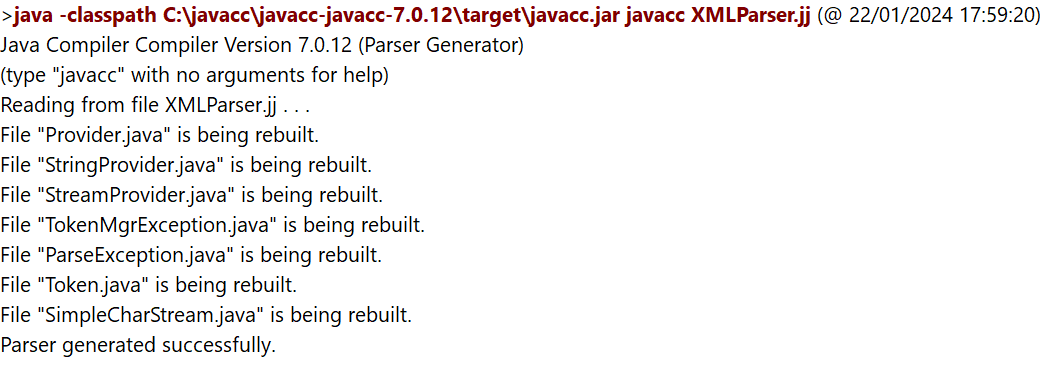
\includegraphics[width=0.9\textwidth]{imagenes/javacccompilation.png}
\caption{\label{fig:javacccompilation}Compilación de Archivos JavaCC en Eclipse}
\end{figure}
\emergencystretch=1em
\section{Símbolos de Expresiones regulares en JavaCC}
\label{sec:simbolosdeexpresionesregulares}
\lstinline[basicstyle=\large\ttfamily]|+| : El símbolo \lstinline[basicstyle=\large\ttfamily]|+| se usa para indicar que \textbf{un elemento puede aparecer una o más veces}. Por ejemplo, si tienes \lstinline[basicstyle=\large\ttfamily]|A+|, significa que se espera que haya al menos una instancia de \lstinline[basicstyle=\large\ttfamily]|A|, pero puede haber más.

\lstinline[basicstyle=\large\ttfamily]|*| : El símbolo \lstinline[basicstyle=\large\ttfamily]|*| se usa para indicar que \textbf{un elemento puede aparecer cero o más veces}. Por ejemplo, si tienes \lstinline[basicstyle=\large\ttfamily]|B*|, significa que \lstinline[basicstyle=\large\ttfamily]|B| es opcional y puede aparecer cero o más veces.

\lstinline[basicstyle=\large\ttfamily]|?| : El símbolo\lstinline[basicstyle=\large\ttfamily]|?| se usa para indicar que \textbf{un elemento puede aparecer cero o una vez}. Por ejemplo, si tienes \lstinline[basicstyle=\large\ttfamily]|C?|, significa que \lstinline[basicstyle=\large\ttfamily]|C| es opcional y puede aparecer cero o una vez.


\lstinline[basicstyle=\large\ttfamily]|~| : El símbolo \lstinline[basicstyle=\large\ttfamily]|~| se utiliza para \textbf{excluir ciertos caracteres} o elementos. Por ejemplo, \lstinline[basicstyle=\large\ttfamily]|~A| significa cualquier carácter excepto \lstinline[basicstyle=\large\ttfamily]|A|. En una expresión regular, \lstinline[basicstyle=\large\ttfamily]|~| se usa para negar un conjunto de caracteres. Por ejemplo, \lstinline[basicstyle=\large\ttfamily]|~[0-9]| significa cualquier carácter que no sea un dígito del 0 al 9.


\chapter{Código Fuente}
\label{sec:codigofuente}

En este apéndice se presenta el código fuente de los archivos referenciados a lo largo del documento para su estudio. Cabe destacar que se proporciona dicho código con el objetivo de que el lector sea capaz de probar las funcionalidades y aprender mas acerca de las aplicaciones de JavaCC.

No se promueve el plagio y la realización de las prácticas, este simplemente es una de las muchas formas en las que se podrían realizar la prácticas.

La realización de las prácticas y de todos los ejemplos mostrados en este documento se encuentran disponibles en:

\href{https://github.com/m-amaris/tfg/tree/main/eclipse-workspace}{https://github.com/m-amaris/tfg/tree/main/eclipse-workspace}

% A partir de este punto, no quieres mostrar los números de página
\pagestyle{empty}

% Definimos los nuevos márgenes de esta sección
\newgeometry{left=1cm,right=1cm,top=2cm,bottom=1cm}

\section{Mathexp.jj}
\label{sec:mathexp}
\lstset{inputencoding=utf8/latin1}
\lstinputlisting[language=java]{code/mathexp.jj}

\newpage
\section{NL\_Xlator.jj}
\label{sec:nlxlator}
\lstset{inputencoding=utf8/latin1}
\lstinputlisting[language=java]{code/NL_Xlator.jj}

\newpage
\section{Descripción general del sistema de correo electrónico}
\label{sec:P2SistemaCorreo}

\noindent Esta sección se ha extraído del enunciado de la Práctica 2 de PIAT.

\begin{figure}[H]
	\centering
	\includegraphics[width=\textwidth]{imagenes/P2SistemaCorreo.jpg}
	\caption{\label{fig:P2SistemaCorreo.jpg}Arquitectura del sistema de correo electrónico\cite{pdfpractica2} }
\end{figure}

\noindent Los mensajes entrantes desde Internet son recibidos inicialmente por los servidores smtp-in, los cuales se los pasan a los servidores security-in que actúan de filtros de antispam y virus entrantes. Si estos filtros detectan un virus, descartan el mensaje y no lo reenvían. En otro caso, se los pasan a los servidores de almacenamiento de correos user-mailbox. Los mensajes que se consideren spam se etiquetan con una marca que sirve a los servidores user-mailbox para almacenarlos en la carpeta de posible spam de la cuenta del usuario.

Los servidores security-in generan mensajes automáticos de notificación de error para correos que no pueden llegar al destino. Esto sucede cuando intentan entregar un mensaje a un user-mailbox y éste responde que la dirección de destino es inexistente o bien que la cuenta de destino ya ha alcanzado su cuota máxima de espacio de almacenamiento de mensajes. En ese momento envía un mensaje a smtp-in y se notifica este error al remitente través de los servidores smtp-out.

Los usuarios del servicio de correo electrónico envían nuevos mensajes, y respuestas a los mensajes recibidos, por medio de los servidores msa (mail submission agent). Estos pasan los mensajes a los servidores security-out que actúan de filtros de spam y virus salientes. En el caso de que estos filtros detecten algún mensaje de spam o que contenga un virus, lo bloquean con objeto de salvaguardar la reputación del sistema. Finalmente, los mensajes son entregados a los smtp-out para que estos los envíen a la estafeta de destino.

\newpage
\section{Formato de logs. Sistema de correo electrónico (Simplificado)}
\label{sec:logscorreo}
\lstset{inputencoding=utf8/latin1}
\lstinputlisting[language=java]{code/msa1.2020022016.log}

\newpage
\section{Parser.jj}
\label{sec:P2Parser}
\lstset{inputencoding=utf8/latin1}
\lstinputlisting[language=java]{code/Parser.jj}

\newpage
\section{Catalogo.xml (Simplificado)}
\label{sec:catalogoxml}
\lstset{inputencoding=utf8/latin1}
\lstinputlisting[language=XML]{code/catalogo.xml}

\newpage
\section{Catalogo.xsd }
\label{sec:catalogoxsd}
\lstset{inputencoding=utf8/latin1}
\lstinputlisting[language=XML]{code/catalogo.xsd}

\newpage
\section{XMLParser.jj}
\label{sec:XMLParser}
\lstset{inputencoding=utf8/latin1}
\lstinputlisting[language=java]{code/XMLParser.jj}

\newpage
\section{JSONParser.jj}
\label{sec:JSONParser}
\lstset{inputencoding=utf8/latin1}
\lstinputlisting[language=java]{code/JSONParser.jj}

% Volvemos a la geometría por defecto del documento
\restoregeometry

\end{document}